%%%%%%%%%%%%%%%%%%%%%%%%%%%%%%%%%%%%%%%%%%%
%
% szablon pracy licencjackiej 
% korzystający ze stylu pracalicmgr.cls
% 2017.03.01 P. Durka durka@fuw.edu.pl 
% na podstawie pliku J. Żygierewicz 2016
%
%%%%%%%%%%%%%%%%%%%%%%%%%%%%%%%%%%%%%%%%%%%



\documentclass{pracalicmgr}
\usepackage{polski}
\usepackage[utf8]{inputenc}

\usepackage{graphicx}
\usepackage{multicol}
\usepackage{caption}
\usepackage{subcaption}


\usepackage{float}
\graphicspath{ {./images/} }

\usepackage{booktabs} %ladne tabelki
\usepackage{tabularx} %kolumna

\usepackage{placeins}
\usepackage{tikz}

%\newcolumntype{C}{>{\centering\arraybackslash}X}  %nowe typy kolumn w tabeli
%\newcolumntype{R}{>{\raggedleft\arraybackslash}X}
%\newcolumntype{s}{>{\hsize=.5\hsize}X}

\newcolumntype{R}{>{\centering\arraybackslash\hsize=.22\hsize}X} 
\newcolumntype{C}{>{\centering\arraybackslash\hsize=.13\hsize}X}




\usepackage{esvect} %do zaznaczania wektorow

%\usepackage[round]{natbib}   % omit 'round' option if you prefer square brackets
%\bibliographystyle{plainnat}
\usepackage[maxcitenames=2, backend=biber, style=authoryear, uniquelist=false]{biblatex}
\renewcommand*{\nameyeardelim}{\addcomma\space}
%\renewcommand*{\nameyeardelim}{\addcomma\space}

\usepackage{ gensymb }

\renewcommand{\contentsname}{Table of contents}
\renewcommand{\listtablename}{List of tables}
\renewcommand{\listfigurename}{List of figures}
\renewcommand{\chaptername}{Chapter}
\renewcommand{\tablename}{Table}
\renewcommand{\figurename}{Figure}
\renewcommand{\appendixname}{Appendix}
\renewcommand{\abstractname}{Summary}



\author{Agnieszka Wierzbicka}

\nralbumu{323371}


\title{Analysis of laminar profile of evoked potentials in rat visual cortex}

\tytulang{Analiza profilu warstowego potencjałów wywołanych w korze wzrokowej szczura}

\kierunek{Zastosowania fizyki w biologii i medycynie}

\specjalnosc{Neuroinformatyka}

\opiekun{Dra hab. Jarosława Żygierewicza,
	\\Zakład Fizyki Biometycznej
	\\Instytut Fizyki Doświadczalnej
	\\Wydział Fizyki, Uniwersytet Warszawski
	\\oraz
	\\Prof. dr hab. Wioletty Waleszczyk,
	\\Pracownia Neurobiologii Widzenia
	\\Zakład Neurofizjologii
	\\Instytut Biologii Doświadczalnej im. Nenckiego, PAN }

%\dziedzina{13.200}
\dziedzina{13.2 Physics}

\date{Grudzień 2017}



\keywords{electrophysiology, visual system, primary visual cortex, visual stimulation, local field potential, current source density, temporal frequency}

\bibliography{bibliografia}

\begin{document}


    \maketitle
    \let\cleardoublepage\clearpage
    
    \begin{abstract}
    In this work responses to visual stimulation with 6 different temporal frequencies from range 1--12 Hz were analyzed. Stimuli (flashing LED light) were applied in 5-second-long series with random (2--3 s) breaks between them. Results from selected channels were presented as averaged potentials, power spectra and current source density which allowed to find differences in laminar profile. For low frequencies $i.e.$ 1 and 2 Hz in averaged potentials there is a clear repolarization in layer IV of primary visual cortex. For higher frequencies in amplitude of  peaks in fundamental frequency and second harmonic in power spectra the following tendency could be observed: upper- and lowermost channels exhibit low amplitudes, while highest amplitudes are reached in the middle channels. Difference between low and high frequencies are also visible in current source density. For 1 and 2 Hz there is a change in polarization by each repetition of stimulus. For stimulation with higher frequency sinks and sources are distinguishable only during first 1.5 s but just after  stimulation, there is a clear change of polarization.

     \end{abstract}

  
    \tableofcontents
    
    \chapter*{Goal}
    \addcontentsline{toc}{chapter}{Goal}
    
    The main goal of this work was to study the responses of neurons from particular layers of the visual cortex to visual stimulation with different temporal frequencies. Several works have been recently published in this field, either focusing on single layer using multiple stimuli (\cite{cooke_bear}), or analyzing the complete profile but with single stimulus only (\cite{maier2011}). The aim of this work was to combine these approaches---analyze multiple layers using multiple stimuli---in order to obtain the complete laminar profile of primary visual cortex.
    

   \chapter{Introduction}
   
   \section{Structure of the visual system}
   Visual perception is an ability to process information coded by light. There are two largely independent visual pathways. Both begin in the retina where light is converted into electrical discharges by photoreceptors and then the information is transferred to ganglion cells and then further via the optic nerve (Fig.~\ref{rys:neural_circuitry}). Here the pathways split. The first one, known as geniculate visual pathway, leads via the dorsal part of lateral geniculate nucleus (LGN) to primary visual cortex (VCx), and from there further to higher-order cortices. The second pathway, known as extrageniculate visual pathway, leads through superior colliculus and the lateral posterior nucleus-pulvinar complex and then---similarly to the first pathway--- the higher-order cortices (\cite{viola, thomsonlayer6}). 
   \begin{figure}[htbp]
   	\begin{center}
   		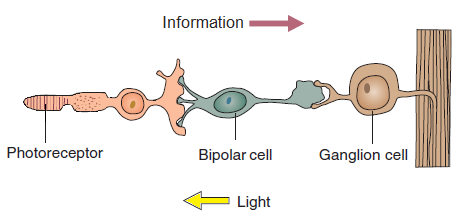
\includegraphics[scale=0.9]{neural_circuitry.png}
   	\end{center}
   	\caption{Neural circuitry in the retina (modified from \cite{carlsonphysiology}).}
   	\label{rys:neural_circuitry}
   \end{figure}      
   
   \section{Parallel processing in the visual system}
   Retina is the first place where visual information is decoded and segregated. Three main morphological types of ganglion cells recognize different properties of visual stimuli (Fig. \ref{rys:ganglio}).
   
   \begin{figure}[H]
   	\begin{subfigure}{.33\textwidth}
   		\centering
   		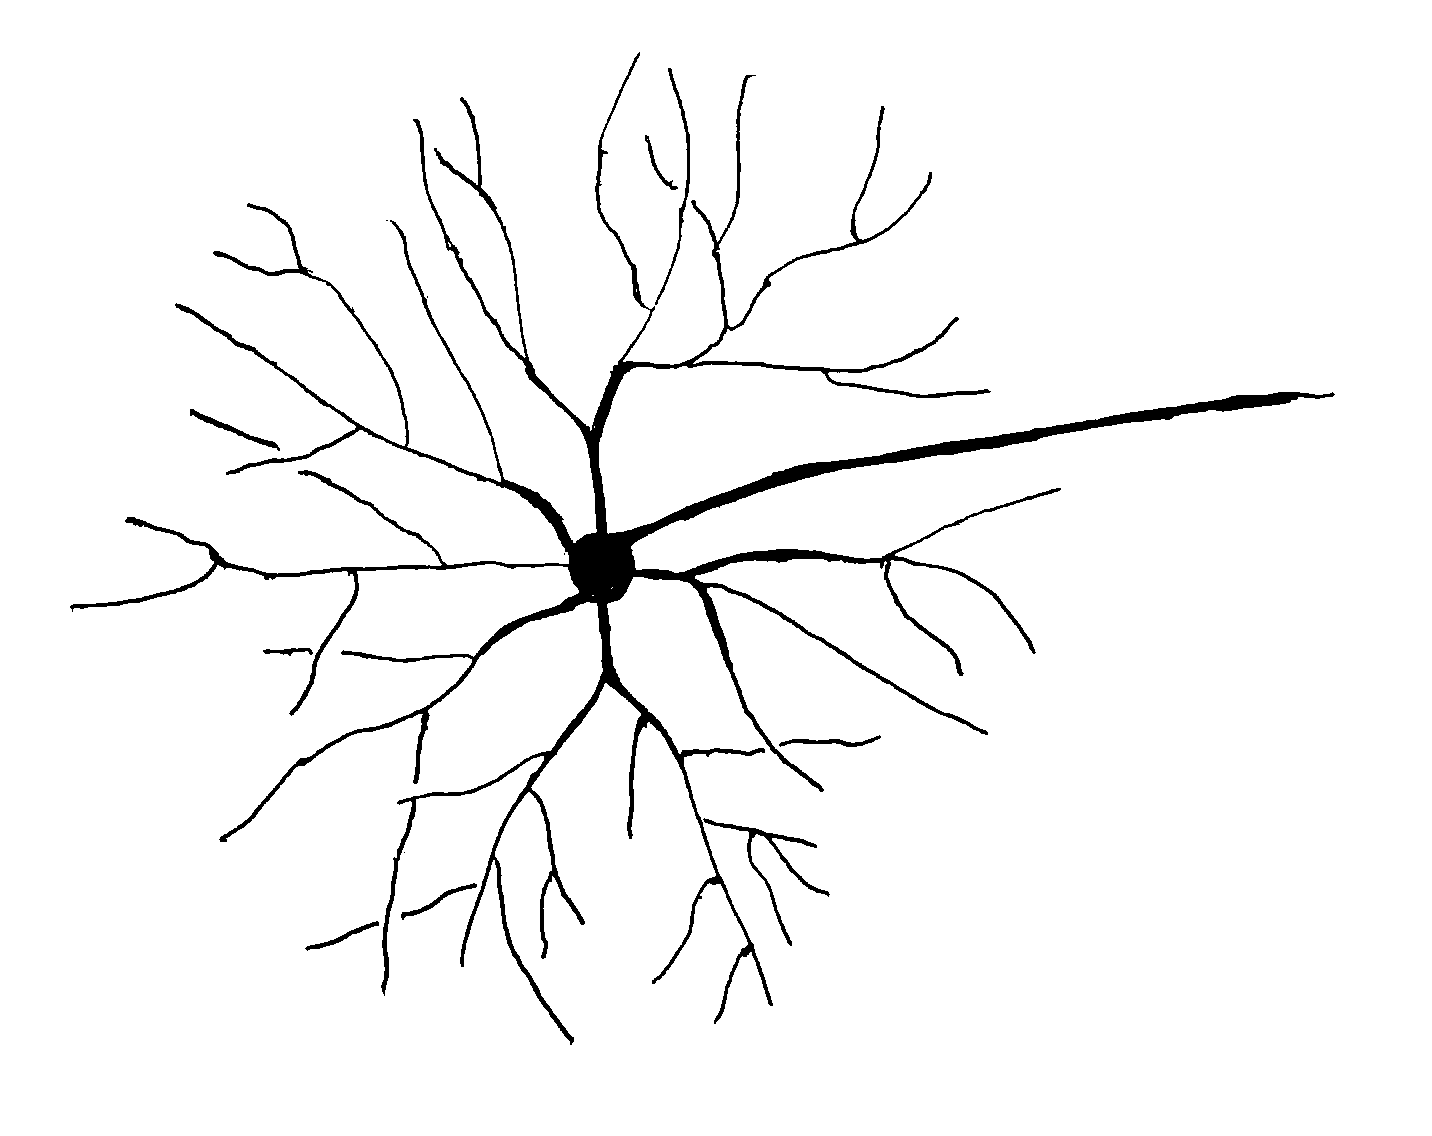
\includegraphics[width=1.\linewidth]{cell_M2.png}
   		\caption{Magnocellular}
   		\label{rys:magno}
   	\end{subfigure}%
   	\begin{subfigure}{.33\textwidth}
   		\centering
   		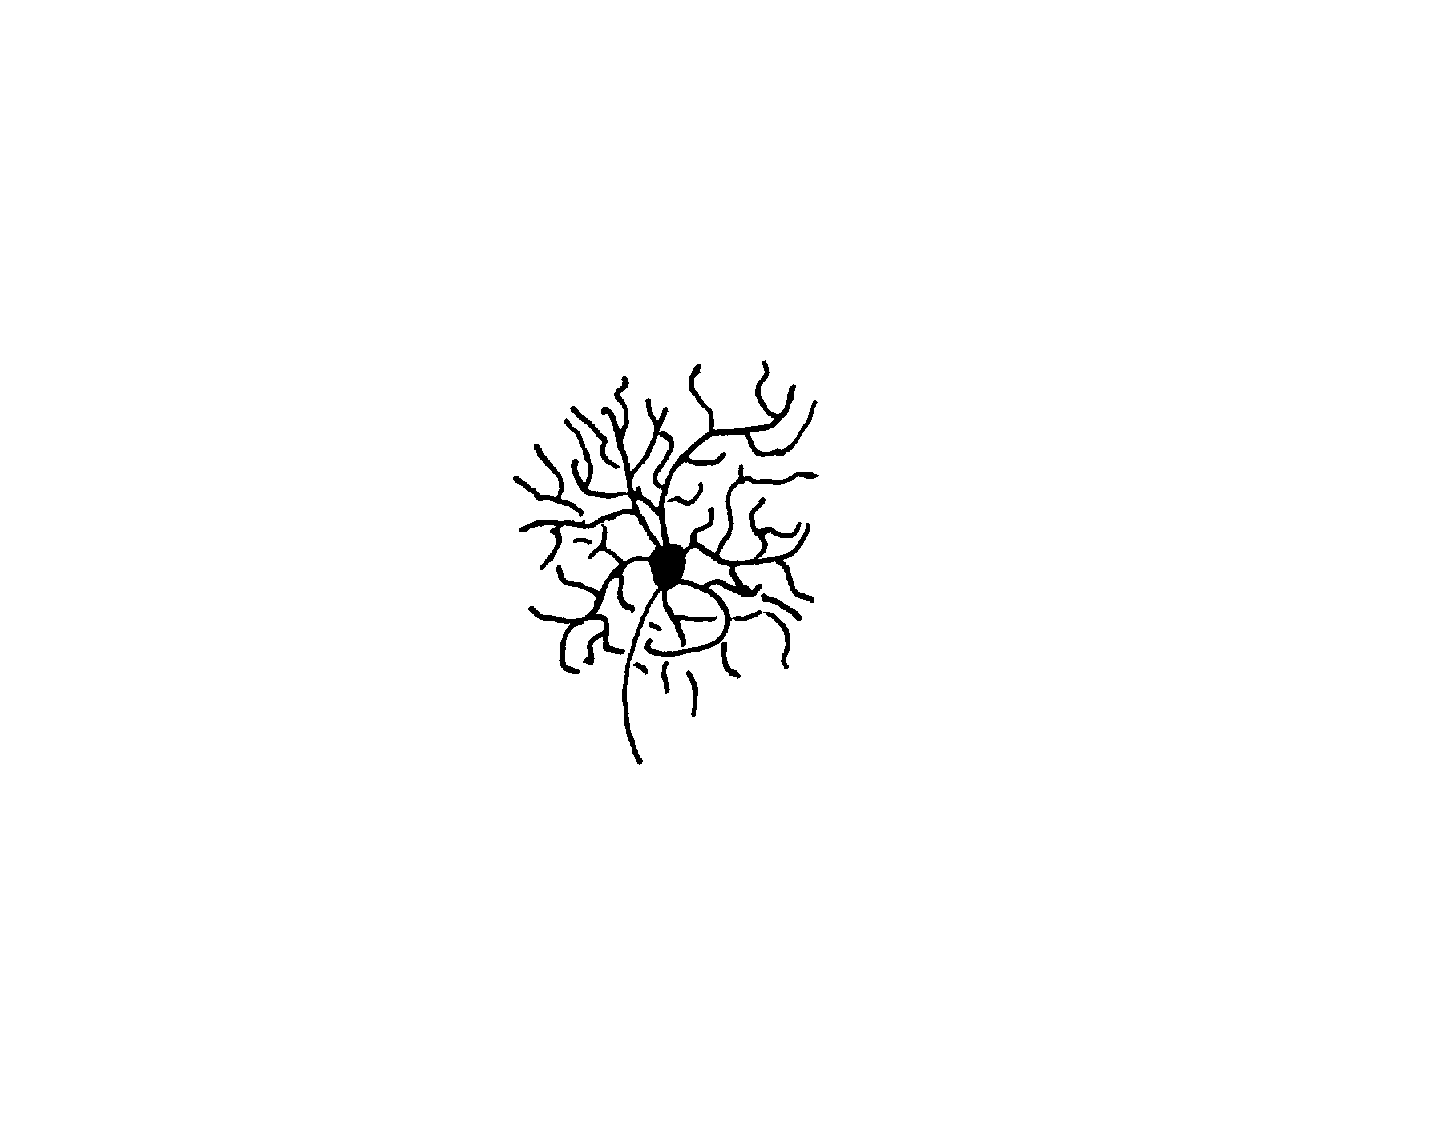
\includegraphics[width=1\linewidth]{cell_P2.png}
   		\caption{Parvocellular}
   		\label{rys:parvo}
   	\end{subfigure}
   	\begin{subfigure}{.33\textwidth}
   		\centering
   		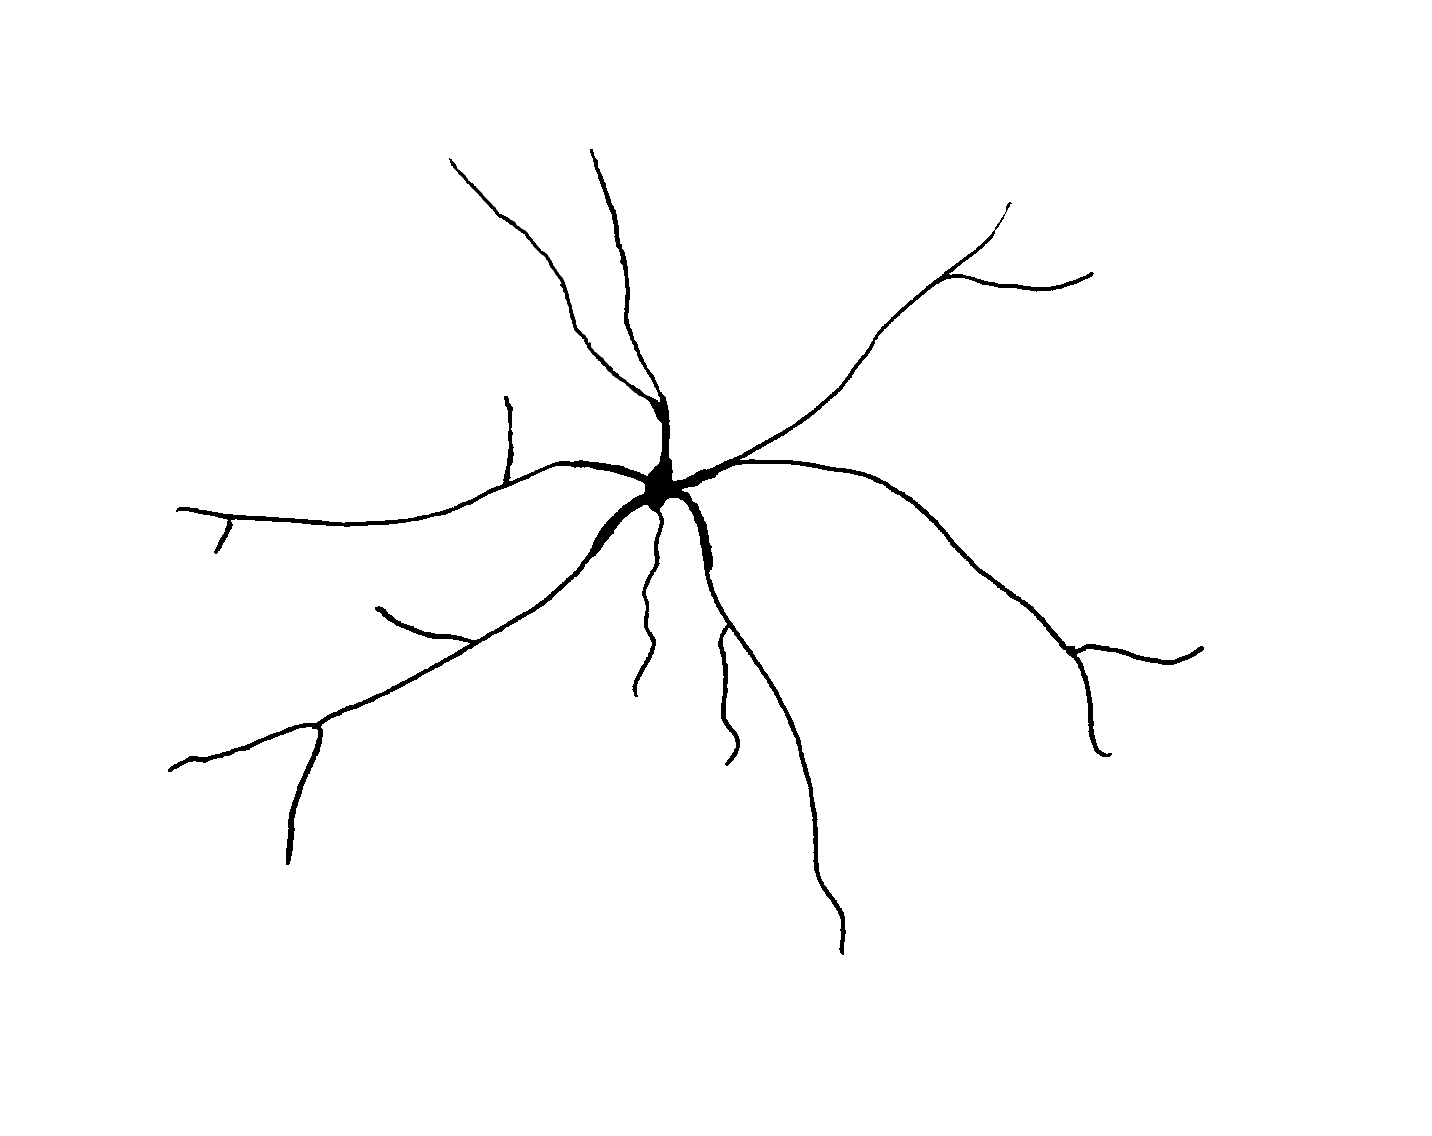
\includegraphics[width=1\linewidth]{cell_K2.png}
   		\caption{Koniocellular}
   		\label{rys:konio}
   	\end{subfigure}
   	\caption{Three most important morphological classes of ganglion cells  (Drawing on the basis of \cite{parallel}).}
   	\label{rys:ganglio}
   \end{figure}
   Magnocellular cells (Fig. \ref{rys:magno}) have big somas with large dendritic trees. Thanks to thick axon, this type of cells can recognize fast stimuli but have poor spatial frequency resolution. Parvocellular cells are cells with medium somas (Fig. \ref{rys:parvo}). They are characterized by high resolution of spatial frequency due to size of dendritic trees, but weak temporal frequency resolution. Koniocellular cells are a heterogeneous group of cells with small-to-medium somata and different dendritic morphologies (Fig. \ref{rys:konio}; \cite{parallel, viola}). 
   
   
   \section{Architecture of the primary visual cortex}
   Primary visual cortex can be divided into six layers differing from one another in function and morphology. Sometimes layers II and III are considered to be one layer II/III. Parallel processing is continued from retina via LGN to VCx. Magnocellular channel enters mainly to layer IV but also to layer VI; parvocellular channel enters layers IV (lower than magnocellular) and VI (higher than magnocellular); koniocellular channel enters layers I, II/III and V (Fig. \ref{rys:lgn}; \cite{parallel}).
   
   \begin{figure}[H]
   	\begin{center}
   		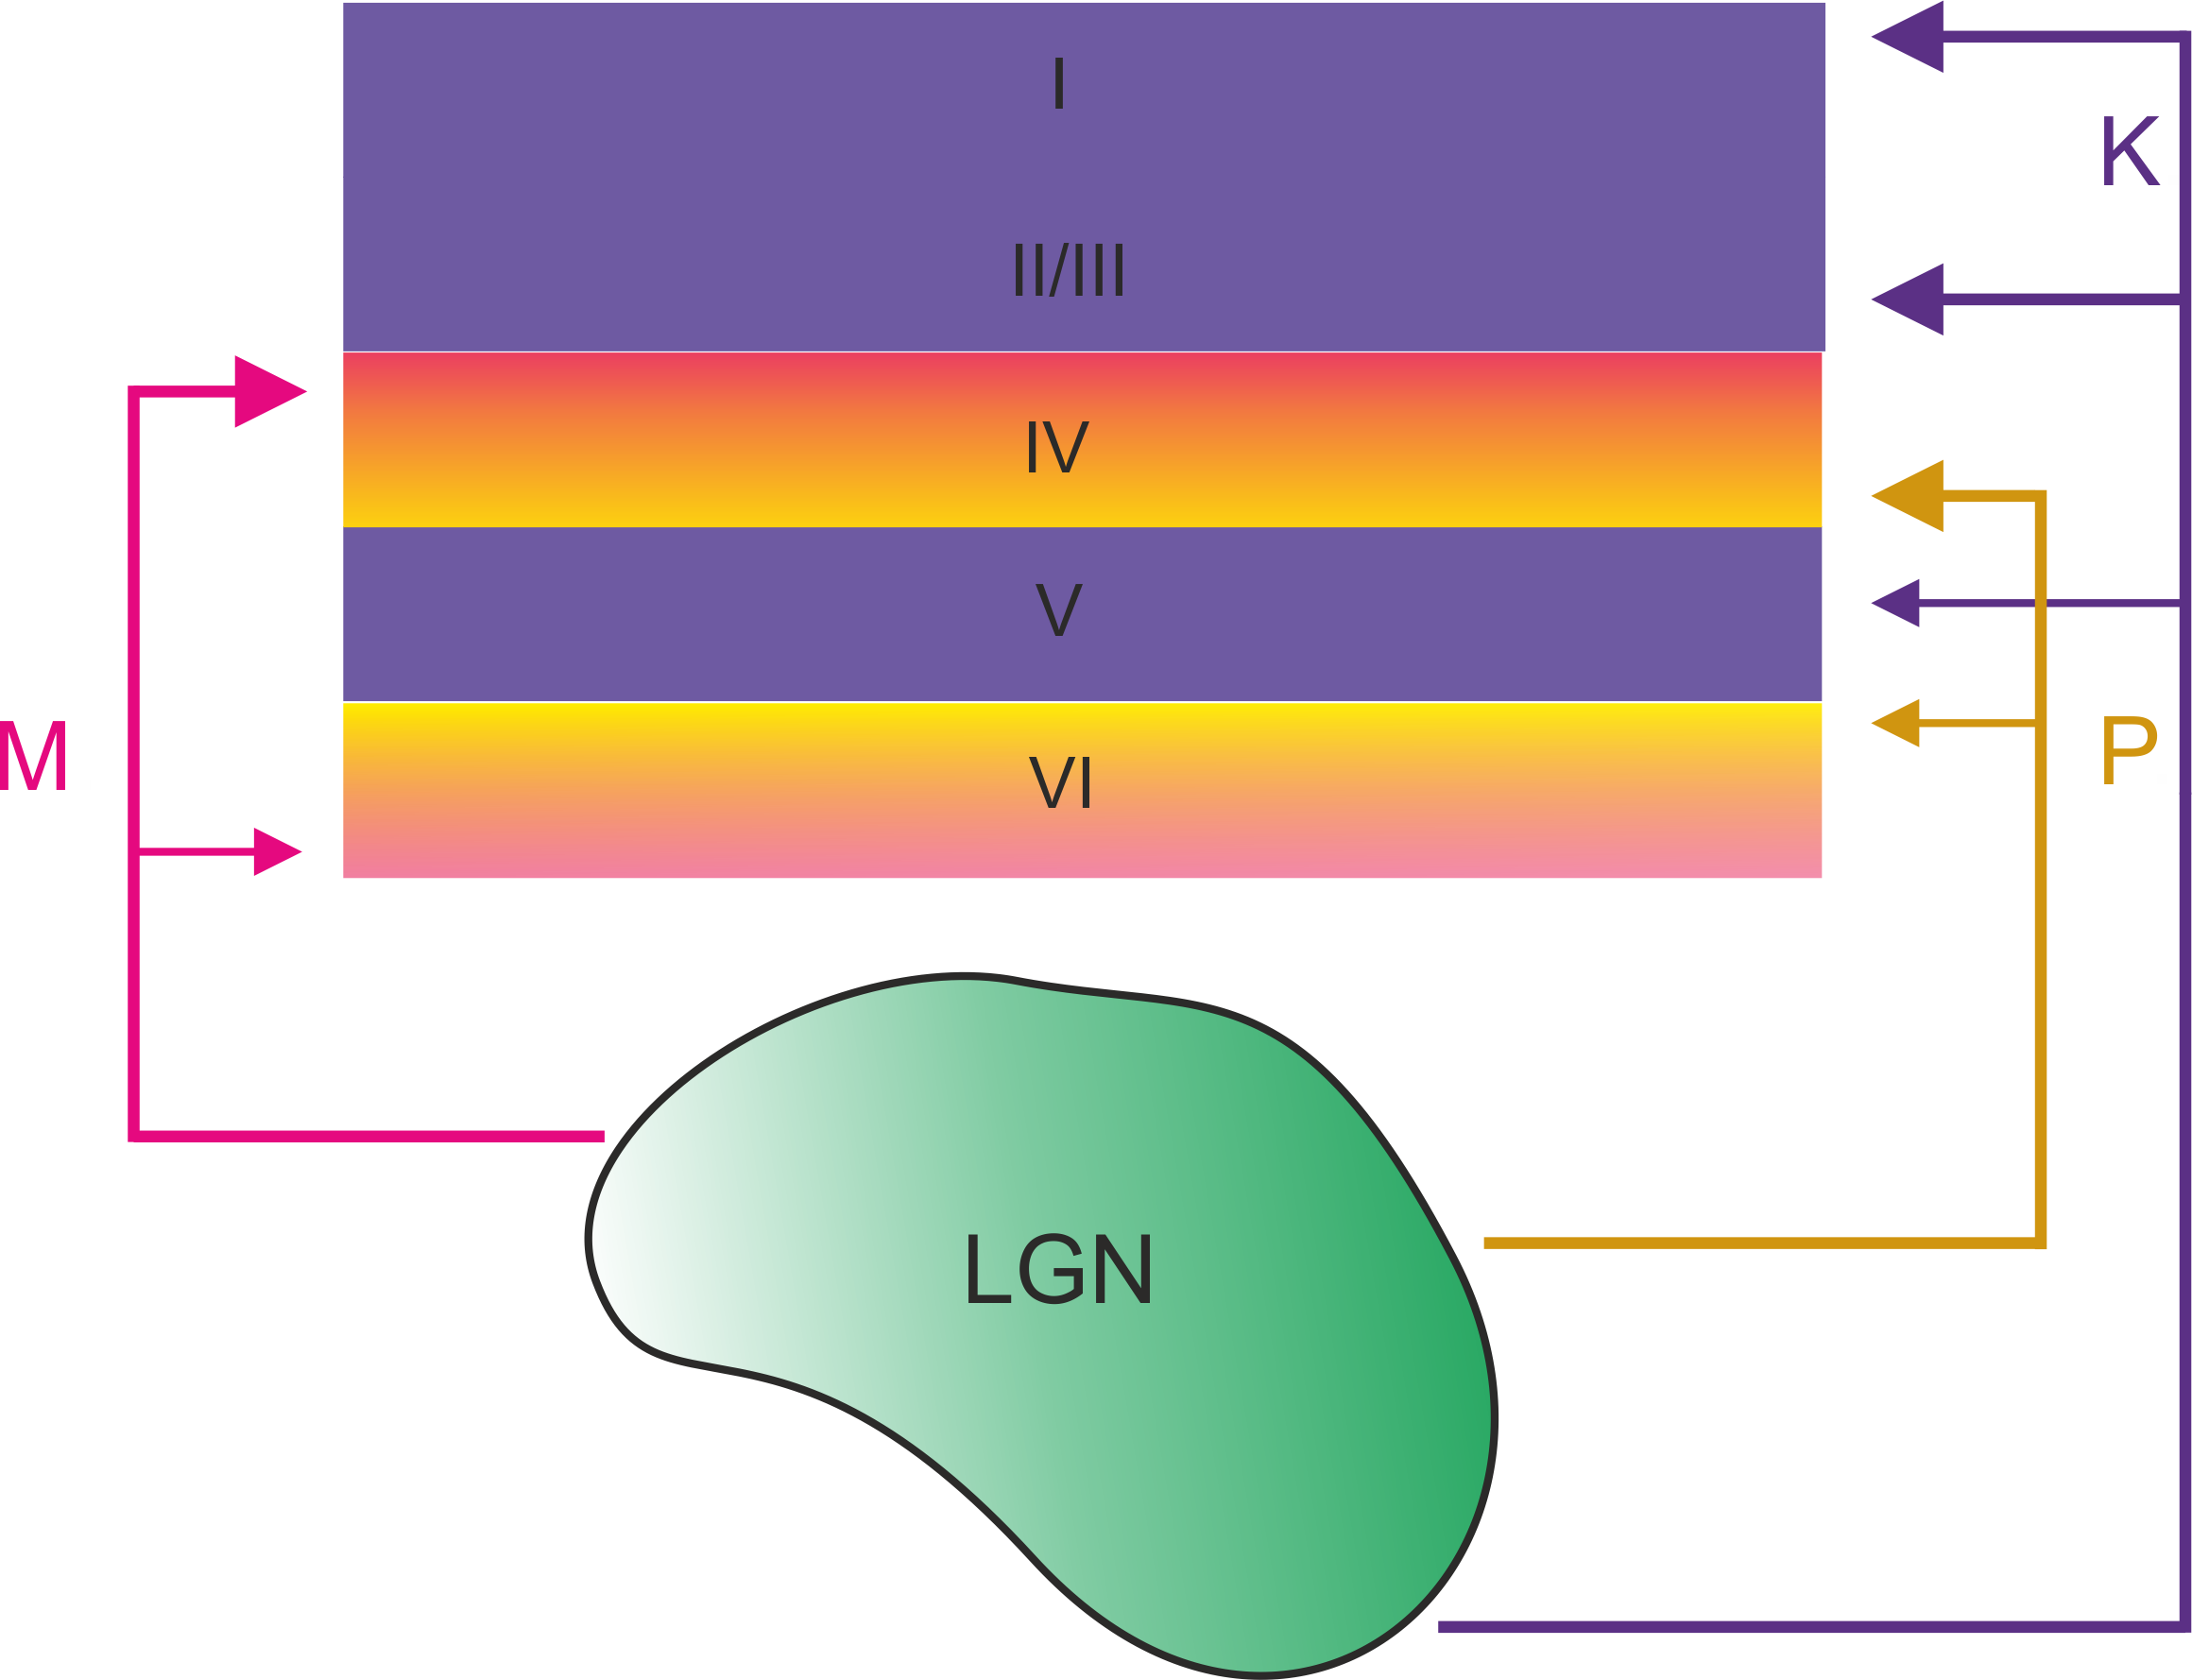
\includegraphics[scale=0.4]{aga_LGN.png}
   	\end{center}
   	\caption{The main connections made by axons from the dorsal lateral geniculate body to primary visual cortex.}
   	\label{rys:lgn}
   \end{figure}  
   \newpage
   Other division can be made based on granule cells located in layer IV. These cells are characterized by very small cell bodies. Layers above layer IV are called \emph{supragranular}, while layers below are referred to as \emph{infragranular}. Around layer IV there is a polarization change observable on averaged evoked potentials (\cite{maier2010}). In layer I cell bodies are absent but there are plenty of axons, dendrites, and synapses. Two major classes of cortical cells are pyramidal cells which occur in all layers except I and IV, and stellate cells which are found in all layers (Fig. \ref{rys:morphology_neurons}).
   
   \begin{figure}[H]
   	\begin{center}
   		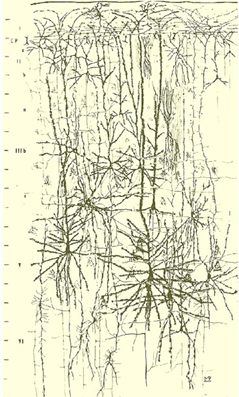
\includegraphics[scale=1]{morphology_neurons.png}
   	\end{center}
   	\caption{Composite figure of a mosaic of camera lucida drawings showing the morphological features (size, location, and distribution) of the principal neuronal types of the human cortex. From rapid-Golgi preparations. Scale (on the left): 100 $\mu$m  (\cite{morphology}).}
   	\label{rys:morphology_neurons}
   \end{figure}   
   
   
   \section{Local field potential}
   Electrophysiology is a method of recording brain activity characterized by high temporal resolution but weaker spatial resolution. Thanks to electrodes inserted in different places in the brain we can gather information from them. Electrophysiology can be used to examine responses to various stimuli at different locations of the brain. Usage of vertical electrodes allows to record simultaneously signal across the brain.
   
   Local field potentials (LFP)---i.e. the low-frequency part of extracellular electrical
   recordings from electrodes inserted into the examined tissue---are a measure of the neural activity reflecting dendritic processing of synaptic inputs to neuronal populations. LFP is a superposition of postsynaptic and action potentials  (Fig. \ref{rys:VCx_LFPs}).
   
   \begin{figure}[H]
   	\begin{center}
   		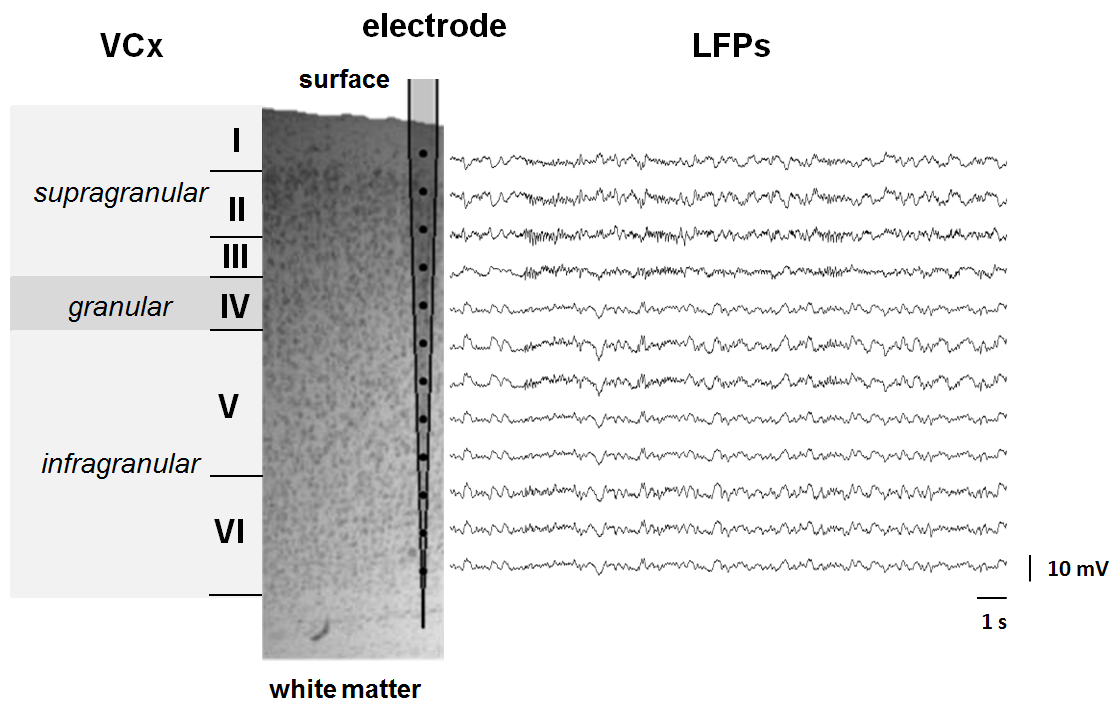
\includegraphics[scale=0.5]{VCx_LFPs2.png}
   	\end{center}
   	\caption{ An example of LFP signals recorded in VCx.}
   	\label{rys:VCx_LFPs}
   \end{figure} 
   
   Postsynaptic potentials are potentials generated in the postsynaptic membrane of a dendrite of a nerve cell. They can be either excitatory (Excitatory Post-Synaptic Potentials, EPSPs)---that enhance chance of induction of action potentials---or inhibitory (Inhibitory Post-Synaptic Potentials, IPSPs)---making action potential less likely to happen. There are lots of potentials reaching every neuron. When the sum of them exceeds a threshold the neuron becomes excited and generates an action potential which propagates along axon (Fig. \ref{rys:PSPs}).
   \begin{figure}[htbp]
   	\begin{center}
   		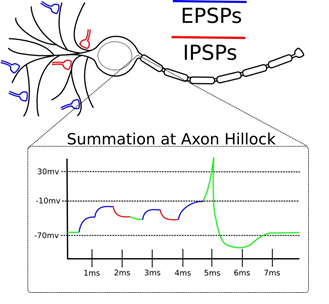
\includegraphics[scale=1]{PSPs.png}
   	\end{center}
   	\caption{Excitatory and inhibitory post-synaptic potentials.}
   	\label{rys:PSPs}
   \end{figure} 
   
   \chapter{Materials and methods}   
   \section{Subjects}
   For electrophysiological experiments presented in this study, we used 6 adult male Wistar rats (250-300g). All animals were housed with free access to food and water and maintained on a 12 h light/dark cycle. All experimental procedures  were conducted in accordance with the ARVO Statement for the Use of Animals in Ophthalmic and Vision Research and  the EC Directive 86/609/EEC for animal experiments using protocols and methods accepted by the First Warsaw Local Ethical Commission for Animal Experimentation. The experiments took place in Laboratory of Visual Neurobiology in Nencki Institute with great help from Katarzyna Kordecka.
   
   
   \section{Surgical procedures}
   Animals under deep urethane anesthesia (1.5 g/kg, Sigma-Aldrich, Germany, 30\% aqueous solution, i.p) were placed in a stereotaxic apparatus. Additional doses of urethane (0.15~g/kg) were administered when necessary. Body temperature was maintained between 36 and 38 \degree C using an automatically controlled electric heating blanket. Every hour fluid requirements were fulfilled by subcutaneous injections of 0.9\% NaCl (1ml/hour) and eyes were humidified with Vidisic (Polfa Warszawa S.A., Poland) to prevent cornea from drying. The skin on the head was disinfected with iodine and local anesthetic 1\% lidocaine hydrochloride (0.5 ml, Polfa Warszawa S.A., Poland) was injected over the scalp. The skull was opened to expose areas of the binocular primary VCx (7.5 mm posterior to bregma, 5.0 mm lateral) in left hemisphere. Coordinates of electrode were chosen based on the rat brain atlas (\cite{atlas}). 
   
   \section{Recording electrode}
   For all experiments the same custom vertical electrode made of tungsten was used (Fig.~\ref{rys:electrode}). The electrode had 12 channels but only recordings from 7 of them were used for analysis. Particular channels of the electrode were chosen independently for each rat and the choice was made after the recording. This procedure was motivated by previous experiments which had shown that it is very difficult to insert the electrode in such a way that a predetermined channel corresponds to layer IV. The cause for this difficulty is that layer IV is very thin. It is also the reason why upper contacts of the electrode were located more densely (0.1 mm intervals) than the lower ones (0.2 mm intervals).
   
   \begin{figure}[H]
   	\begin{center}
   		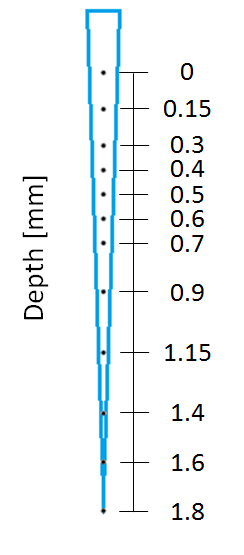
\includegraphics[scale=0.5]{electrode.png}
   	\end{center}
   	\caption{Scheme of 12-channel vertical electrode with intervals between contacts expressed in mm.}
   	\label{rys:electrode}
   \end{figure}
   Although the same electrode was used for all the experiments, the exact depth of each channel varied. This was due to anatomical differences between subjects and imperfect spatial accuracy of the applied method. Therefore channel numbers do not correspond to the same actual physical channels in all experiments. Table~\ref{tab:chosen_chan} presents the exact depth of every channel for every rat. For further explanation of channel choice see Section~\ref{sec:data_prep}.
   \begin{table}[H]
   	\caption{Assignment of channels numbers to actual electrode channels for each animal. Channels without any number were discarded.}
   	\begin{center}
   		\begin{tabularx}{0.9\textwidth}{R C C C C C C C}
   			\toprule
   			\textbf{Depth~[mm]} & \textbf{Rat1} & \textbf{Rat2} & \textbf{Rat3} & \textbf{Rat4} & \textbf{Rat5} & \textbf{Rat6} \\
   			\midrule
   			0 & 1 & 1 & 1 & 1 & 1 & 1 \\
   			0.15 &  &  & 2 & & 2&  \\
   			0.3 & 2 & 2 &  & 2 & & 2 \\
   			0.4 &  &  & 3 &  &  &  \\
   			0.5 & 3 & 3 &4  & 3 & 3 & 3 \\
   			0.6 & & 4 &  & 4 & & 4 \\
   			0.7 & 4 &  &  &  & 4 &  \\
   			0.9 & & 5 & 5 & 5 & 5& 5 \\
   			1.15 & 5 &  &  &  & 6 & 6 \\
   			1.4 & & 6 & 6 & 6 & 7 &  \\
   			1.6 & 6 &  &  &  & & 7 \\
   			1.8 & 7 & 7 & 7 & 7 & &  \\
   			\bottomrule
   		\end{tabularx}
   	\end{center}
   	\label{tab:chosen_chan}
   \end{table}
   \newpage
   \section{Stimulation procedure}
   In the experiments stimuli were presented with interstimulus intervals of  1, 0.5, 0.25, 0.2, 0.143, 0.08 [s] which correspond to frequencies 1, 2, 4, 7, 10, 12 [Hz], respectively. An individual stimulus was a 2-millisecond-long LED flash at 560 cd/m$^2$ luminance. It was dark in the room and rats had both eyes opened. For each frequency the stimuli were applied in 40 repetitions of 5-second-long series with random (2-3 s) breaks between them (Fig. \ref{rys:stimuli}).
   \begin{figure}[htbp]
   	\begin{center}
   		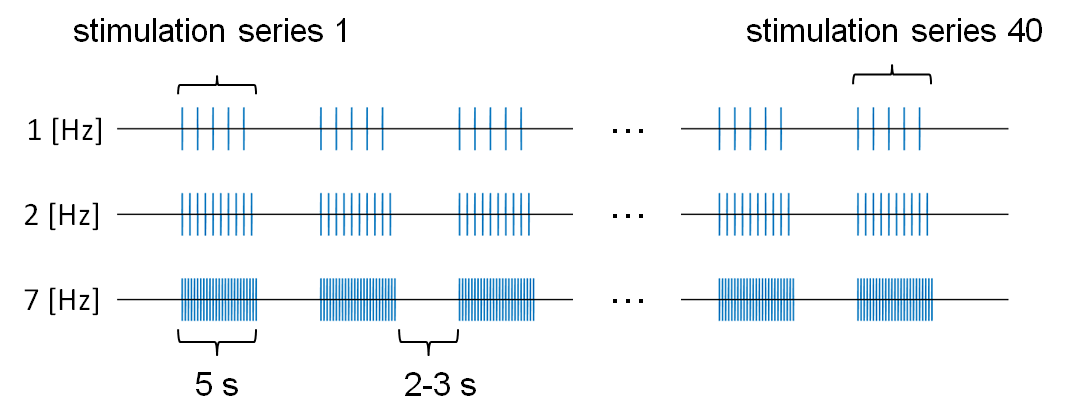
\includegraphics[scale=0.5]{paradigms.png}
   	\end{center}
   	\caption{ Stimulation protocol. The stimuli were presented in 5 s long 40 series at given frequency (from 1 to 12 Hz). The number of stimuli in a series depended on frequency.}
   	\label{rys:stimuli}
   \end{figure} 
   
   \chapter{Data analysis}
   
   \section{Data preparation}
   \label{sec:data_prep}
   Signal was filtered by a bandpass filter in range of 0.3--500 Hz with 500 gain using differential AC amplifiers (A-M 140 Systems, US) and recorded with sampling frequency 1000 Hz. For further analysis hardware filter turned out to be insufficient so three other Butterworth filters were used: 1\textsuperscript{st} order lowpass at cut off 100 Hz,  1\textsuperscript{st} order bandstop at cut off between 45 and 55 Hz and  1\textsuperscript{st} order highpass at cut off 0.5 Hz. To avoid change of phase of the signal \textit{filtfilt} function was used. After filtering each channel of data was normalized by subtracting the mean of all recordings for each channel and divided by their standard deviation. Butterworth filters were used because they are characterized by low deformation of signal giving smooth and monotonic transfer function. It is at cost of low efficiency of filtering, but for this data it was sufficient. After this preparation data was cut into 6-s-long chunks from -0.5~s to 5.5~s where 0 corresponded to the beginning of stimulation and averaged across trials. For further analysis 7 channels out of 12 from contralateral (in respect of stimulation side) VCx were chosen to obtain representative profile: 3 of supragranular, 3 of infragranular and one channel from granular layer (layer IV; Fig \ref{rys:kanaly}).
   
   \begin{figure}[H]
   	\begin{center}
   		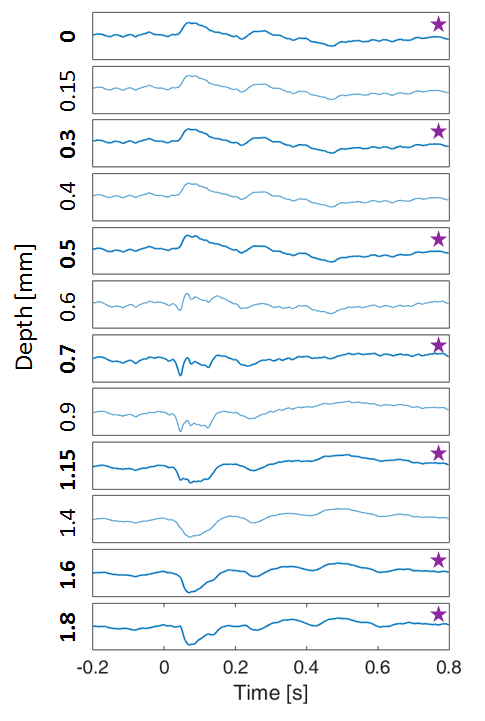
\includegraphics[scale=0.75]{wybieranie_kanalow3.png}
   	\end{center}
   	\caption{ Averaged evoked potentials from VCx from Rat1. On channels at 0.6 and 0.7~mm depth repolarization can be observed. Channels chosen to further analysis are marked by purple stars. Time 0 s means an occurrence of stimulus. Y axis the same for all subfigures.}
   	\label{rys:kanaly}
   \end{figure} 
   
   Reducing the number of channels was necessary due to two reasons:
   \begin{itemize}
   	\item sometimes short circuits between channels occurred,
   	\item there were differences of depth of electrodes and layer IV was recorded by different channels.
   \end{itemize} 
   
   The choice was made based on analysis of the averaged evoked potentials. The referential depth was established by a channel where repolarization was observed right after the occurrence of the stimulus. This channel was assumed to be recorded from layer IV. Then 3 other channels above the reference and 3 more below were chosen, possibly maximally scattered, but avoiding channels which exhibited any distortion. This method is a simplified version of the one introduced by (\cite{maier2011}).
   
   
   \section{Averaging of visual potentials}
   
   \subsection{Description of the method}
   Visual Evoked Potential (VEP) is a case of steady state evoked potential where light is the stimulus. Theoretically, spontaneous activity of ECoG is a stochastic process (independent, stationary noise with mean equal to zero) and brain response to each stimulus is constant. 
   Assuming this signal in each realization can be expressed as follows:
   \begin{equation}
   x_i(t) = s(t) + n_i(t),
   \end{equation}
   where $s(t)$ is a real signal, $n_i(t)$ noise part. For white noise with mean zero, expected value equals:
   \begin{equation}
   E\left[ \frac{1}{N}\sum_{i=1}^{N} n_i(t)\right] = 0, 
   \end{equation}
   which in turn for averaged signal gives us:
   \begin{equation}
   E\left[ \bar{x}(t) \right] = s(t)
   \end{equation}
   
   The effect of averaging is shown in Figure \ref{rys:usrednianie}. Visual response to a single visual stimulus is usually too weak to distinguish it from the background of spontaneous activity of visual cortex. Averaging across several repetitions makes evoked potential stand out.
   \begin{figure}[H]
   	\begin{center}
   		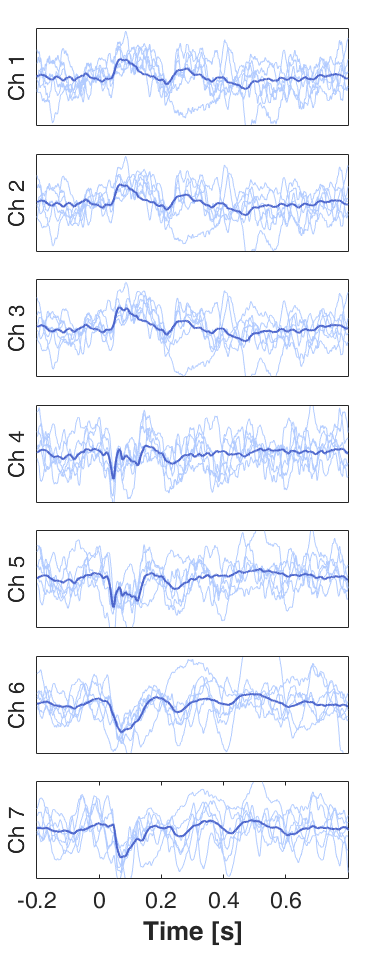
\includegraphics[scale=0.6]{usrednianie3.png}
   	\end{center}
   	\caption{ Comparison between single trials and their average for Rat1. Lighter blue lines represent few examples of responses to a single repetition of a stimulus. Bold and darker line is the average across all trials. Y axis is the same for all subfigures. }
   	\label{rys:usrednianie}
   \end{figure} 
   
   \subsection{Measurement of peak amplitude in VEP}
   For stimulation with frequencies 1 and 2 Hz it was possible to observe visual evoked potentials. There were always two deflections from zero: first almost immediately after the stimulus and second about 0.3~s later (Fig. \ref{rys:wybor_pikow}). Further they are called first and second peak (no matter whether they are negative or positive).
   \begin{figure}[H]
   	\begin{center}
   		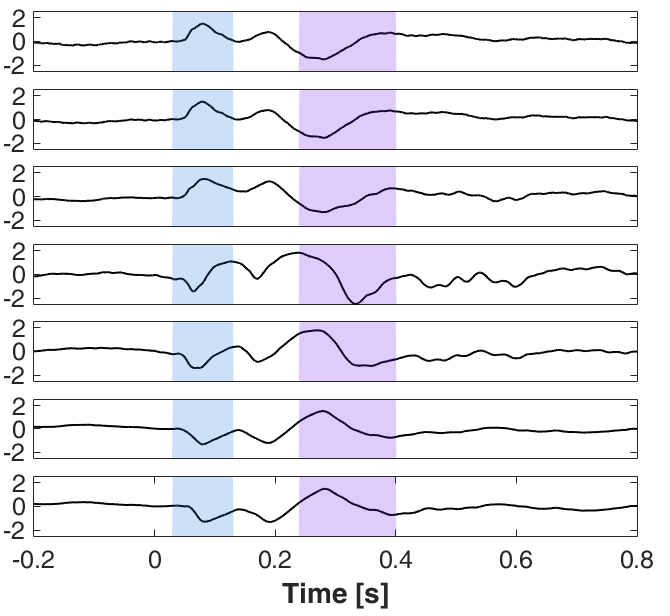
\includegraphics[scale=0.55]{wybor_pikow.png}
   	\end{center}
   	\caption{Averaged potentials for Rat4 stimulated with 1 Hz. Amplitude of the first peak was calculated for the period marked with blue background (0.03--0.13~s after stimulus). Amplitude of the second peak was calculated for the period marked with purple background (0.24--0.4~s after stimulus).}
   	\label{rys:wybor_pikow}
   \end{figure} 
   
   In Figure~\ref{rys:amplitude} first channel for the same rat as in Figure~\ref{rys:wybor_pikow} is presented. Amplitude was taken to be the most extreme value (i.e. having the highest absolute value) in a specified time after an occurrence of a stimulus.
   \begin{figure}[H]
   	\begin{center}
   		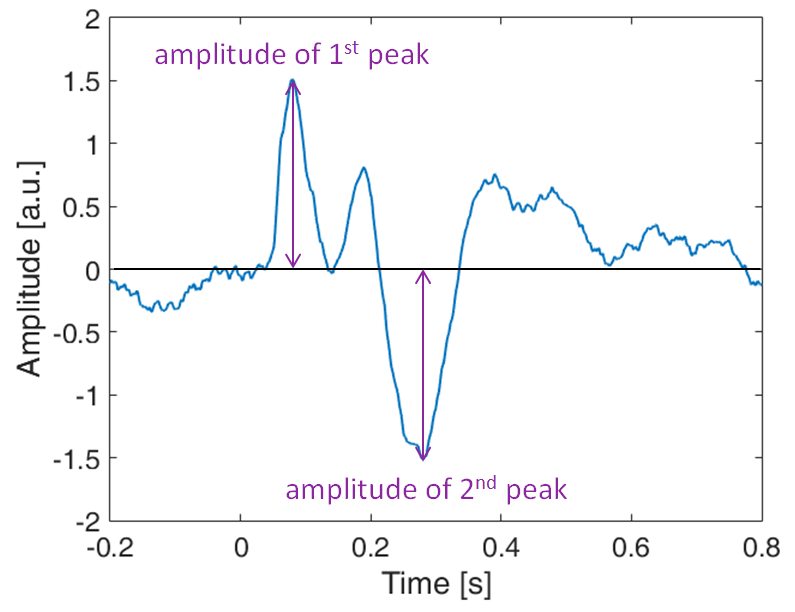
\includegraphics[scale=0.5]{amplitude2.png}
   	\end{center}
   	\caption{Measurement of the peaks amplitude for channel 1 of Rat4 stimulated with 1~Hz. }
   	\label{rys:amplitude}
   \end{figure} 
   
   
   \section{Estimation of signal spectrum}
   Spectra of the signals were estimated by a method introduced by Welch (\cite{welch}). It relies  on splitting the signal into overlapping time windows, estimation of the periodogram for each of the windows, and then averaging of the estimates. In this experiment, data was averaged by 5-second-long chunks for 7 channels and estimation of power spectrum density was calculated. 3-second-long Hamming window with overlap of 2 seconds was used. In Figure \ref{rys:pik_widmo} measurement of the amplitude of fundamental frequency and second harmonic is presented. Amplitudes are the exact values of power spectrum in specific frequencies. 
   
   \begin{figure}[H]
   	\centering
   	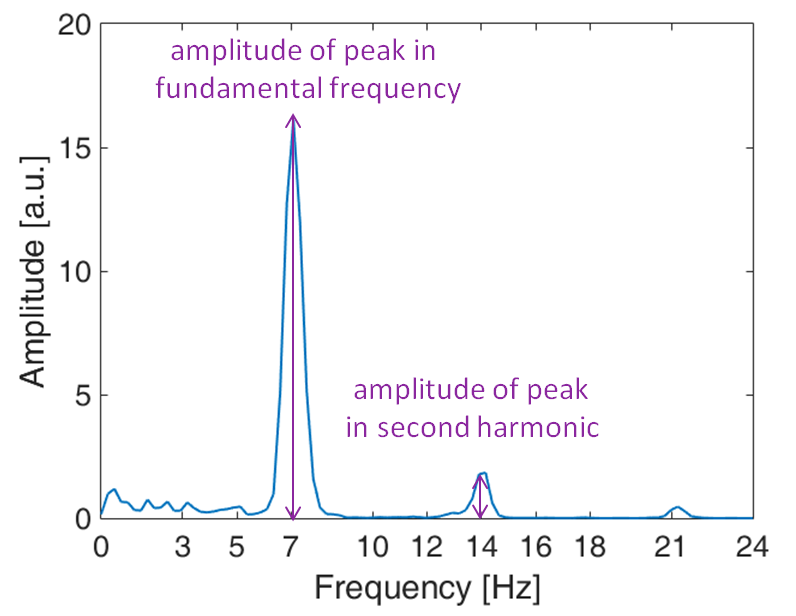
\includegraphics[scale=0.5]{pik_widmo2.png}
   	\caption{Measurement of the peak amplitude for channel 1 of Rat4 stimulated with 7~Hz.}
   	\label{rys:pik_widmo}
   \end{figure}
   
   
   \section{Current Source Density}
   To localize synaptic dynamics it is convenient, whenever possible, to estimate the density of transmembrane current sources (CSD) generating the LFP. Let us assume that we record potential in infinitive, homogeneous and isotropic conductive medium. Current $I$ in that tissue has current density $\vv{J}$ given by equation:
   \begin{equation}
   \vv{J}= \frac{I \vv{r}}{4\pi r^2}
   \end{equation}
   radially at a distance $r$ from the source. In conductive medium with conductivity $\sigma$ Ohm's law describes relation between current density and potential:
   \begin{equation}
   \vv{J}=-\sigma \nabla V.
   \end{equation}
   Multitude of currents $I_j$ located at $\vv{r_j}$ induce potential:
   \begin{equation}
   V(\vv{r})=\sum_{j} \frac{I_j}{4 \pi \sigma |\vv{r}-\vv{r'}|} .
   \end{equation}
   Introducing current source density equals to:
   \begin{equation}
   C(\vv{r})=\sum_{j} I_j \delta (\vv{r}-\vv{r'}),
   \end{equation}
   we can find a relation between potential and CSD:
   \begin{equation}
   V(\vv{r})=\frac{1}{4\pi\sigma}\int d^3 \vv{r'} \frac{C(\vv{r'})}{|\vv{r}-\vv{r'}|},
   \end{equation}
   where $V$ is potential generated by sources, $\sigma$ is a conductivity, $\vv{r}$ is a distance between potential and source. By inverting this relation we get Poisson equation:
   \begin{equation}
   C(\vv{r})=-\sigma \Delta V.
   \label{eq:2}
   \end{equation}
   Equation \ref{eq:2} can be generalized for arbitrary conductivity tensor fields $\sigma$:
   \begin{equation}
   C(\vv{r})=-\nabla \cdot [\sigma \nabla V].
   \end{equation}
   In this work to calculate CSD the method introduced by Jan Potworowski called \textit{kernel Current Source Density} (kCSD) was used (\cite{potworowski, wojcik}).
    
    \chapter{Results}
	In Sections \ref{sec:time} and \ref{sec:freq} all results were presented in the same way. On Figure~\ref{rys:przyklad_odch} an example of used method is shown on the evoked potentials in channel 4 of Rat1.
	
	\begin{figure}[H]
		\centering
		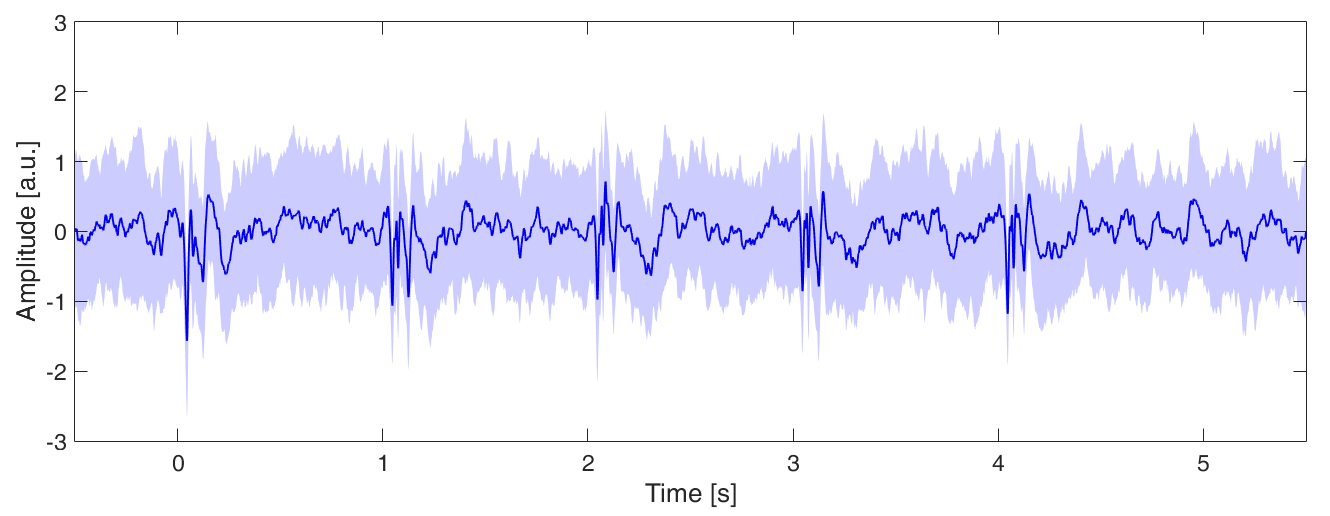
\includegraphics[width=1.\linewidth]{przyklad_odch2.png}
		\caption{Method of presenting results on an example of stimulation of 1 Hz in time domain. Bold line is the average evoked potential for all animals and blue background is the dispersion from the mean by one standard deviation. }
		\label{rys:przyklad_odch}
	\end{figure}

    \section{Overview of results obtained in the time domain}
    \label{sec:time}
    Next, there are all experiments with 6 different stimulation frequency presented one after another. In the Figure \ref{rys:srednie_1_2} results of stimulation with 1 and 2 Hz frequencies are presented---there is a clear peak of response after each repetition of stimulus.
    
    \begin{figure}[H]
    \begin{subfigure}{.5\textwidth}
	\centering
		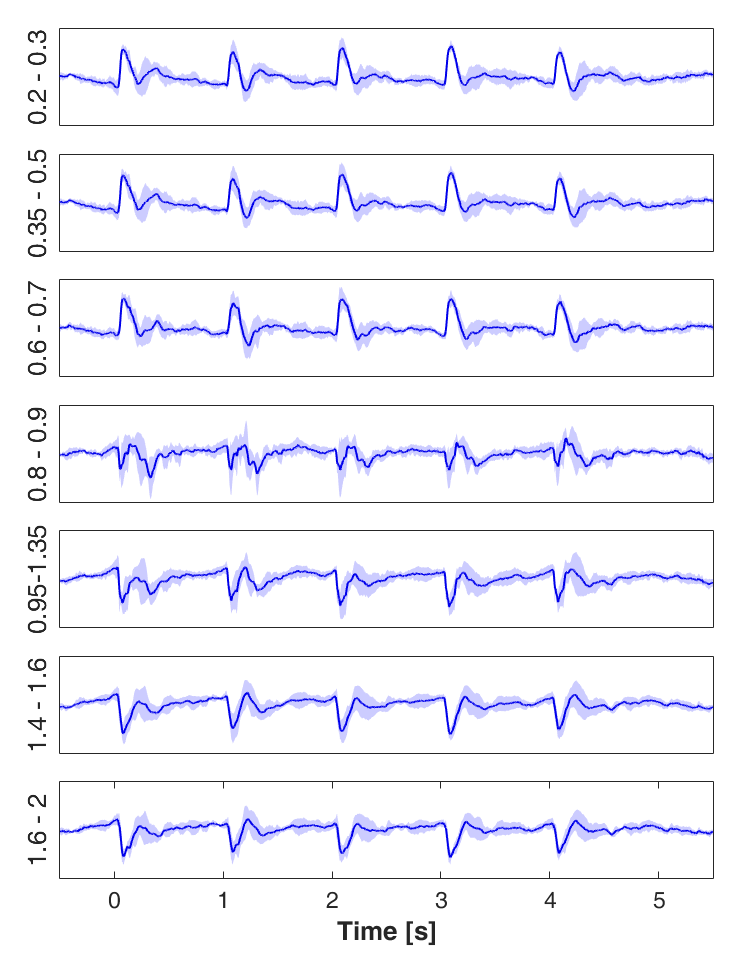
\includegraphics[width=1.\linewidth]{srednie_1Hz_5s.png}
		\caption{Averaged signal for stimulation of 1 Hz.}
		\label{rys:srednie_1Hz}
	\end{subfigure}
	\begin{subfigure}{.5\textwidth}
			\centering
		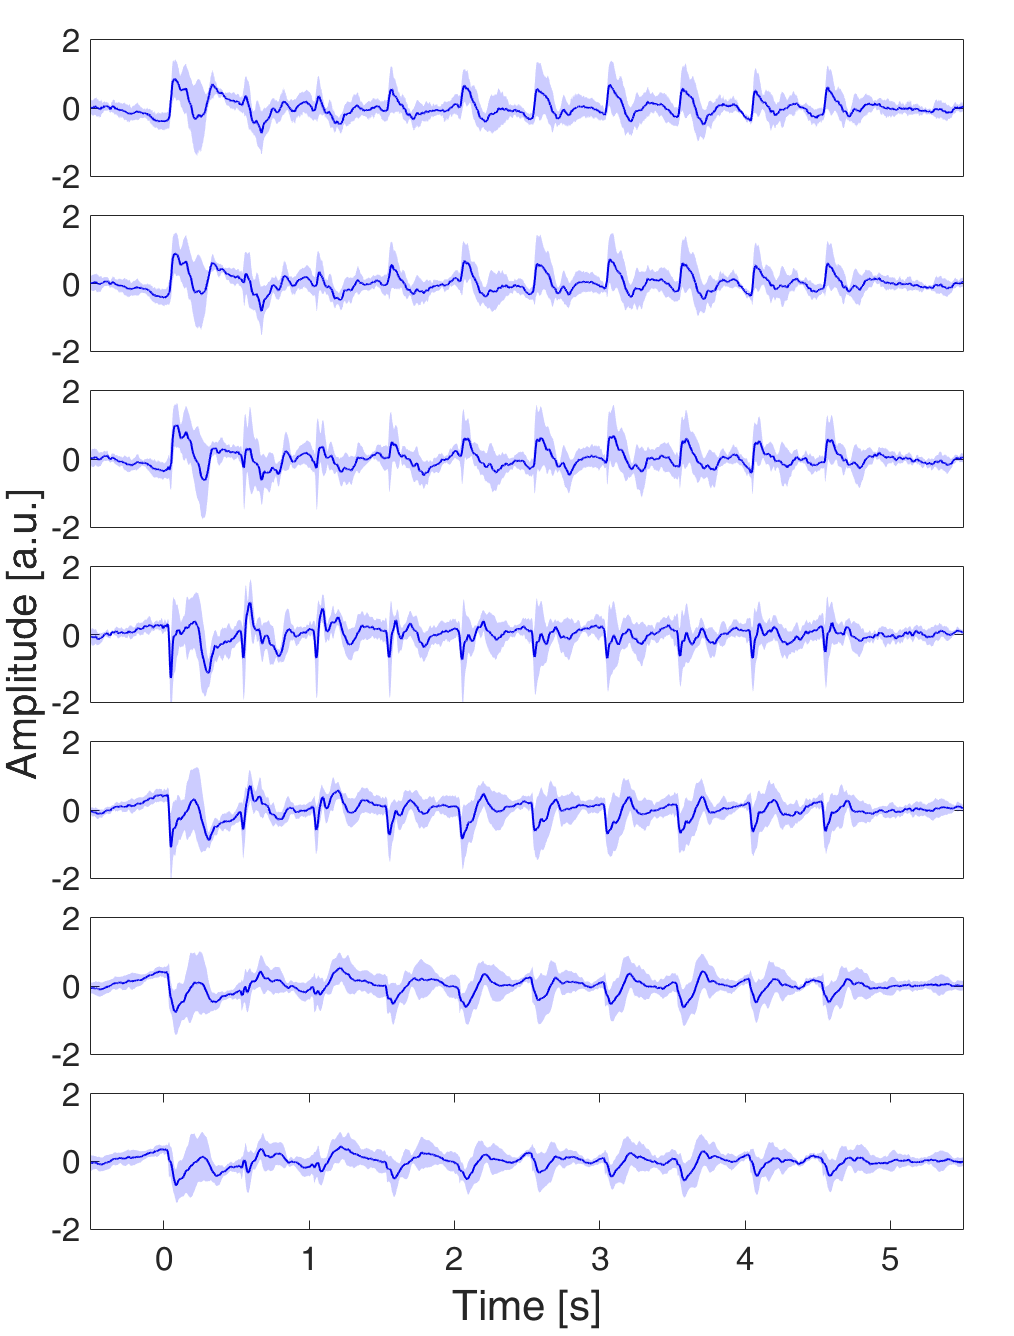
\includegraphics[width=1.\linewidth]{srednie_2Hz_5s.png}
		\caption{Averaged signal for stimulation of 2 Hz.}
		\label{rys:srednie_2Hz}
	\end{subfigure}
	\caption{Results in time domain for stimulation with low frequencies.}
	\label{rys:srednie_1_2}
	\end{figure}
    
    For frequencies higher than 2 Hz signals look different (Fig. \ref{rys:srednia_czas}). Firstly the response for stimuli is blurred: stimuli occurs so often that it is impossible to determine where response for certain stimulus starts and ends. The signal forms a continuous oscillation. During the first 1.5 s of the stimulation: the amplitude of oscillations is higher than for the rest. At around 5.15 s there is noticeable peak probably as a response to end of stimulation. 
    
	\begin{figure}[H]
	\begin{subfigure}{.5\textwidth}
		\centering
		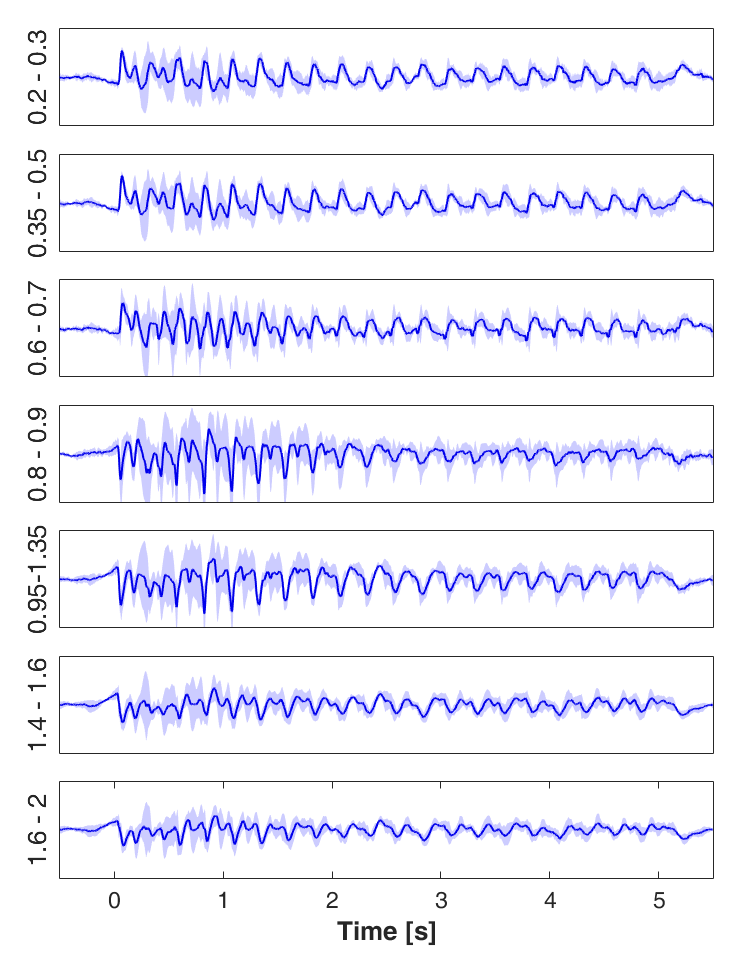
\includegraphics[width=1.\linewidth]{srednie_4Hz_5s.png}
		\caption{Averaged signal for stimulation of 4 Hz.}
		\label{rys:srednie_4Hz}
	\end{subfigure}
	\begin{subfigure}{.5\textwidth}
	\centering
	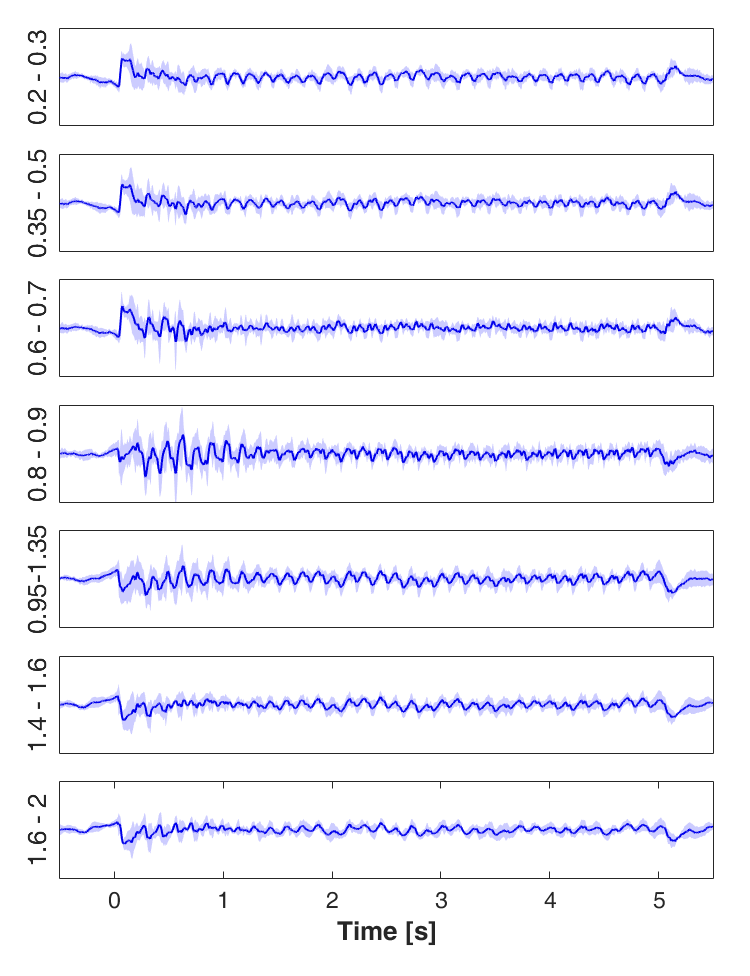
\includegraphics[width=1.\linewidth]{srednie_7Hz_5s.png}
	\caption{Averaged signal for stimulation of 7 Hz.}
	\label{rys:srednie_7Hz}
    \end{subfigure}
	
	\begin{subfigure}{.5\textwidth}
	\centering
	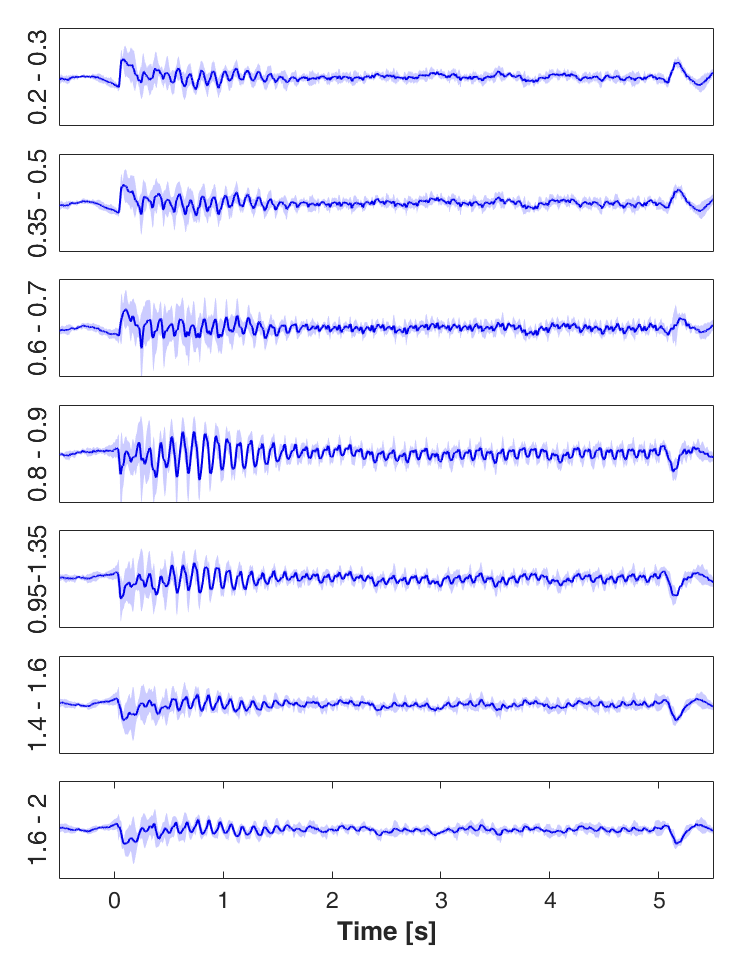
\includegraphics[width=1.\linewidth]{srednie_10Hz_5s.png}
	\caption{Averaged signal for stimulation of 10 Hz.}
	\label{rys:srednie_10Hz}
	\end{subfigure}
	\begin{subfigure}{.5\textwidth}
	\centering
	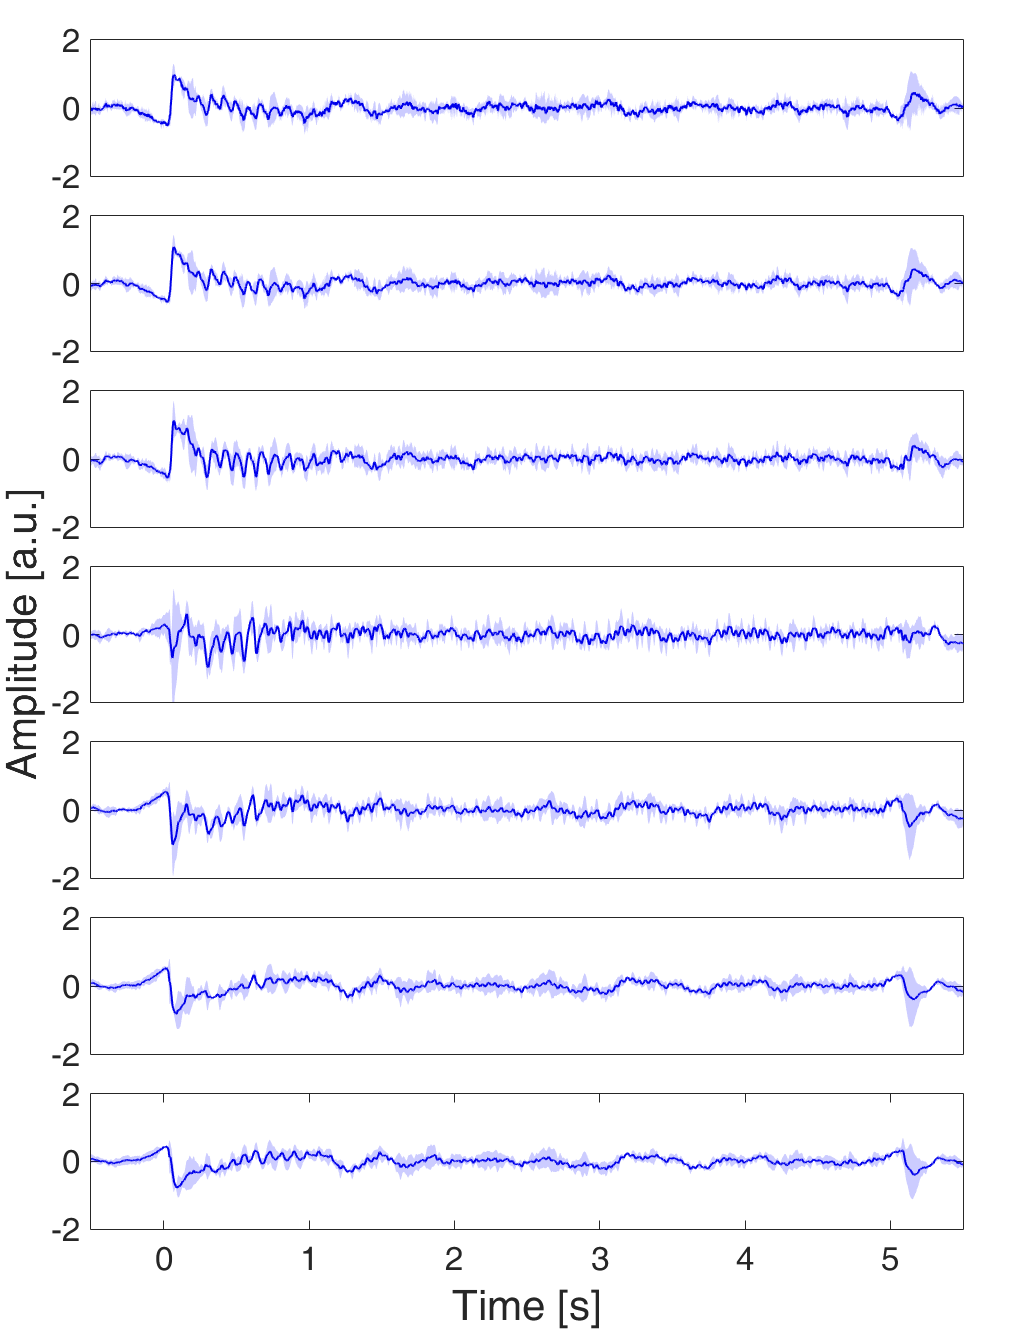
\includegraphics[width=1.\linewidth]{srednie_12Hz_5s.png}
	\caption{Averaged signal for stimulation of 12 Hz.}
	\label{rys:srednie_12Hz}
	\end{subfigure}
	\caption{Results in time domain for stimulation with high frequencies.}
	\label{rys:srednia_czas}
		
	\end{figure}
	
    \section{Overview of results obtained in the frequency domain}
    \label{sec:freq}
    
    Power spectra calculated by Welch's methods are shown in Figures \ref{rys:widmo_1_2} and \ref{rys:srednie_widmo}. For stimulation of 1 Hz there are up to 5 harmonic, and for both 1 and 2 Hz there is so high dispersion that for lowest values there is no difference between peak and zero (Fig. \ref{rys:widmo_1_2}).     
    
    \begin{figure}[H]
    	\begin{subfigure}{.5\textwidth}
    		\centering
		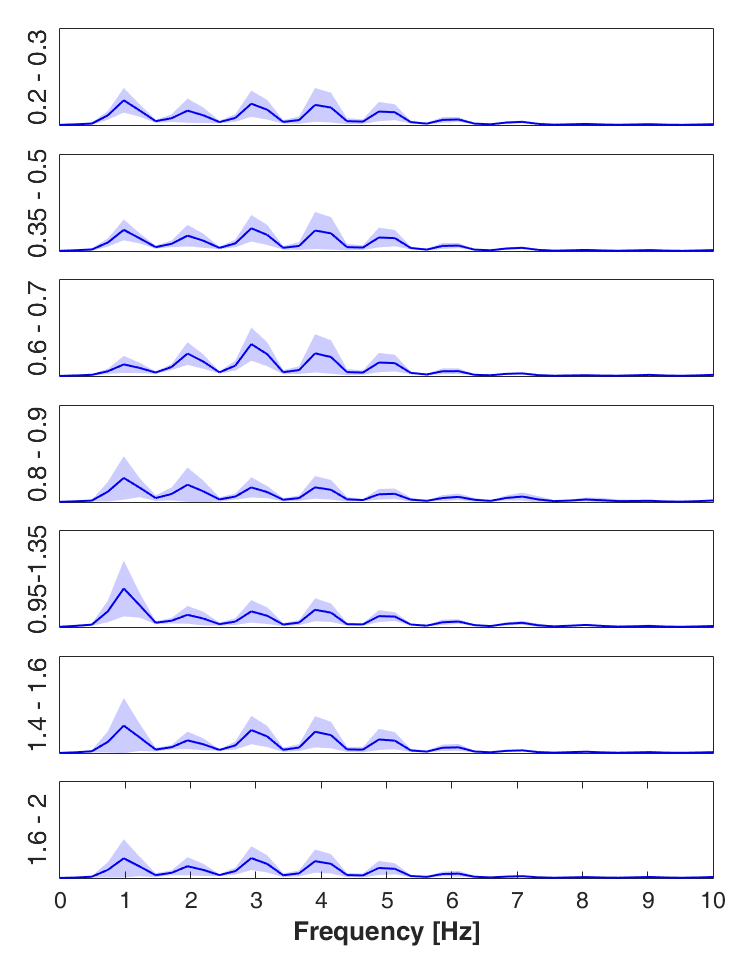
\includegraphics[width=1.\linewidth]{widmo_1Hz.png}
		\caption{Power spectrum for stimulation of 1 Hz.}
		\label{rys:widmo_1Hz}
    	\end{subfigure}
    	\begin{subfigure}{.5\textwidth}
    		\centering
		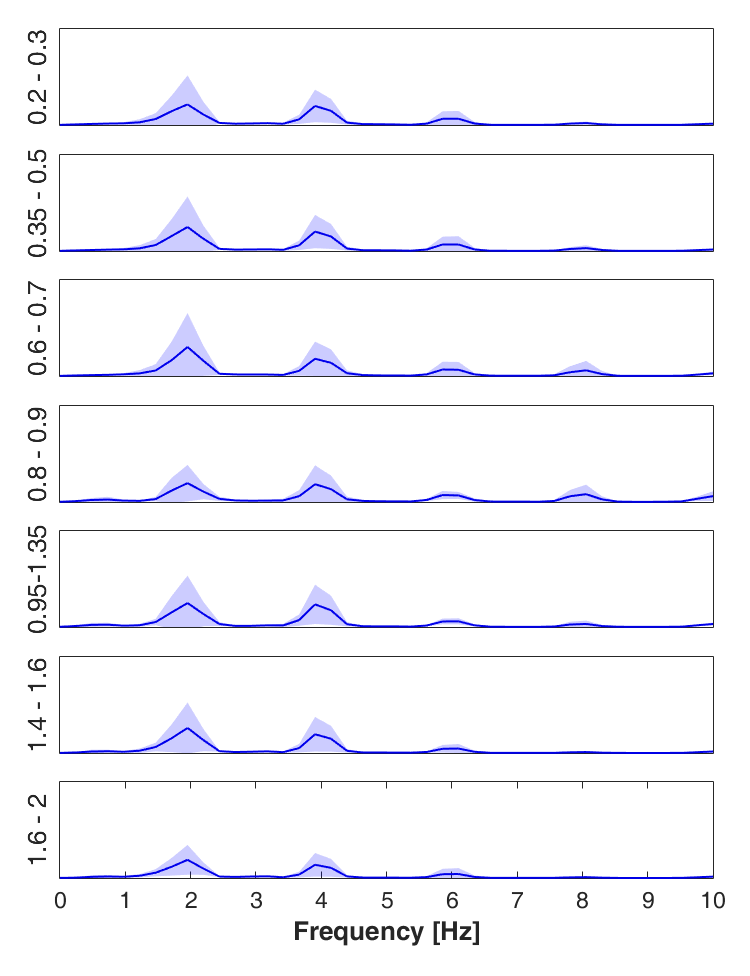
\includegraphics[width=1.\linewidth]{widmo_2Hz.png}
		\caption{Power spectrum for stimulation of 2 Hz.}
		\label{rys:widmo_2Hz}
    	\end{subfigure}
    	\caption{Results in frequency domain for stimulation with low frequencies.}
    	\label{rys:widmo_1_2}
    \end{figure}
    
    For frequencies from range 4 -- 10 Hz, the fundamental frequency and the second harmonic are clean and much bigger than others. Response for 12 Hz in power spectrum is noticeably weaker -- peak in the fundamental frequency is at the same level as low frequency noise (Fig.~\ref{rys:srednie_widmo}).
    
	\begin{figure}[H]
	\begin{subfigure}{.5\textwidth}
		\centering
		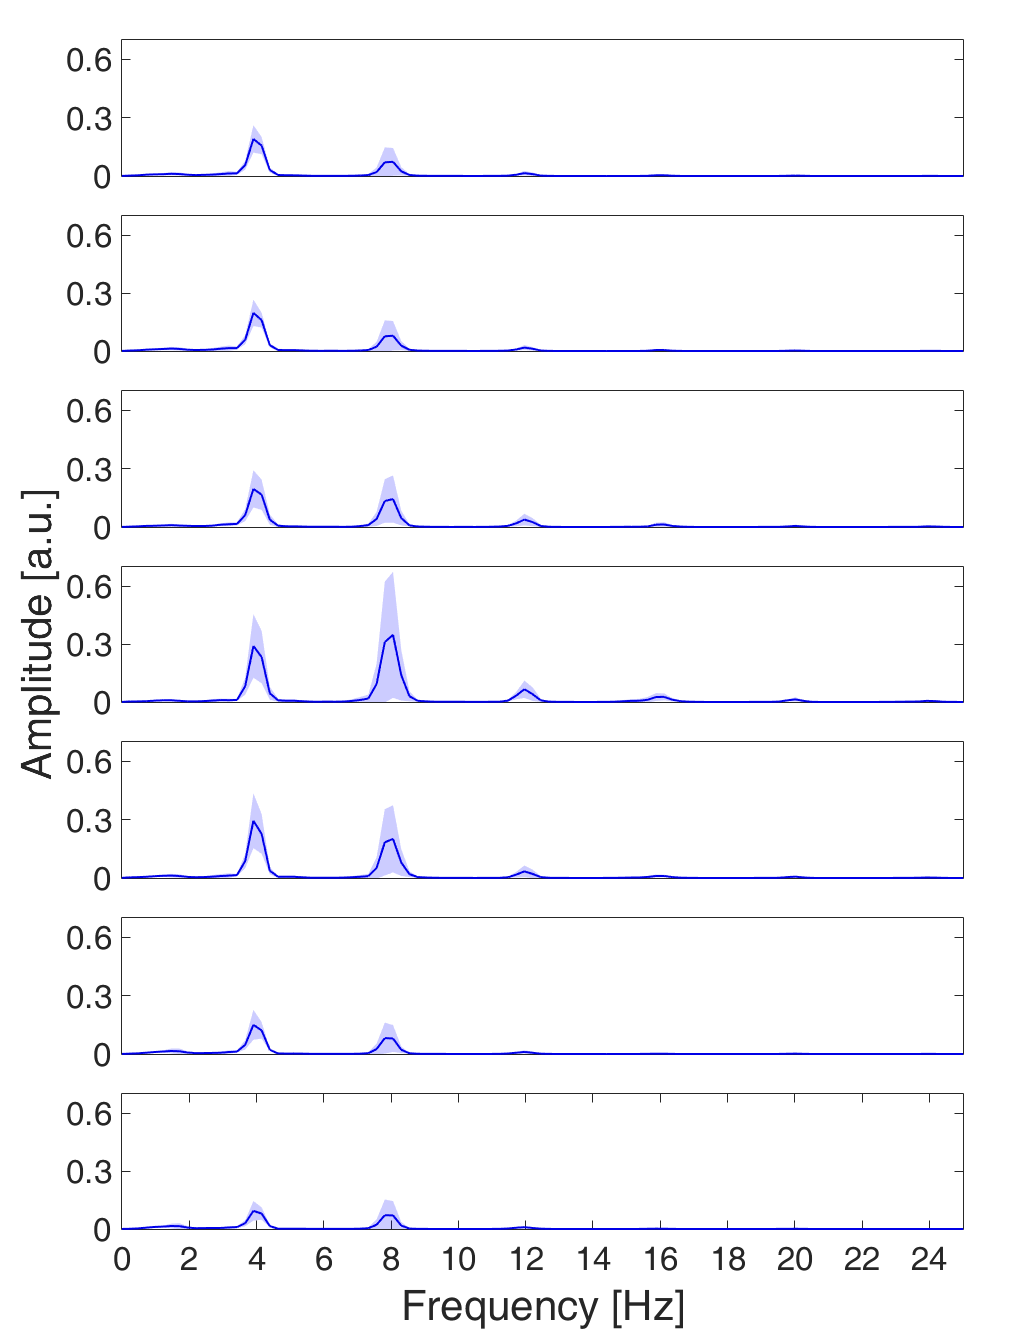
\includegraphics[width=1.\linewidth]{widmo_4Hz.png}
		\caption{Power spectrum for stimulation of 4 Hz.}
		\label{rys:widmo_4Hz}
	\end{subfigure}
	\begin{subfigure}{.5\textwidth}
		\centering
		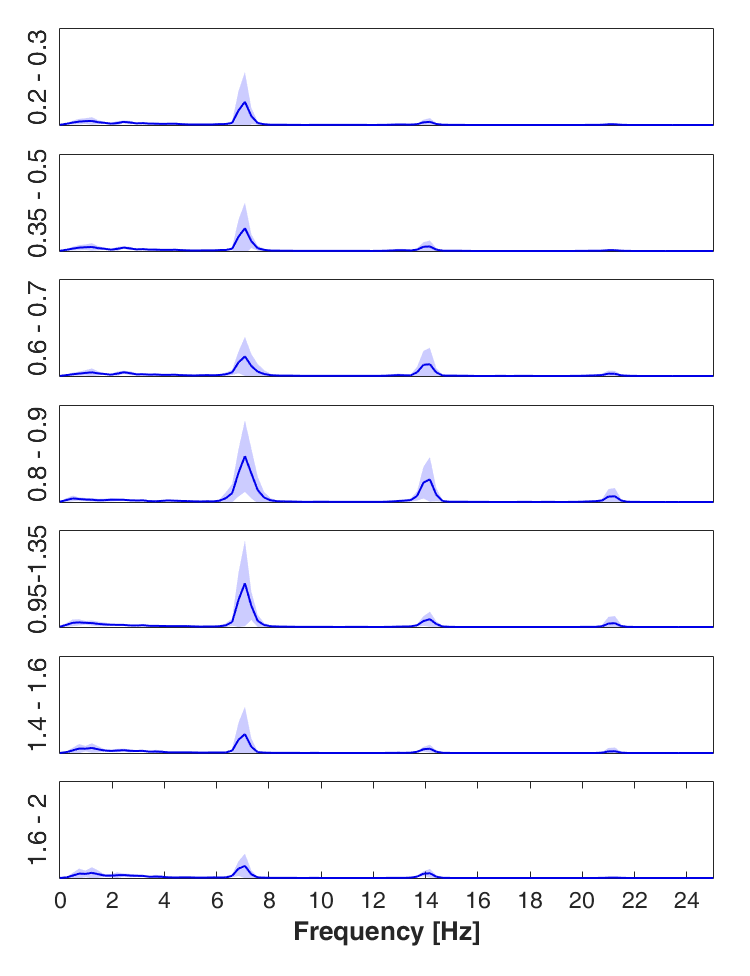
\includegraphics[width=1.\linewidth]{widmo_7Hz.png}
		\caption{Power spectrum for stimulation of 7 Hz.}
		\label{rys:widmo_7Hz}
	\end{subfigure}
		
		
	\begin{subfigure}{.5\textwidth}
		\centering
		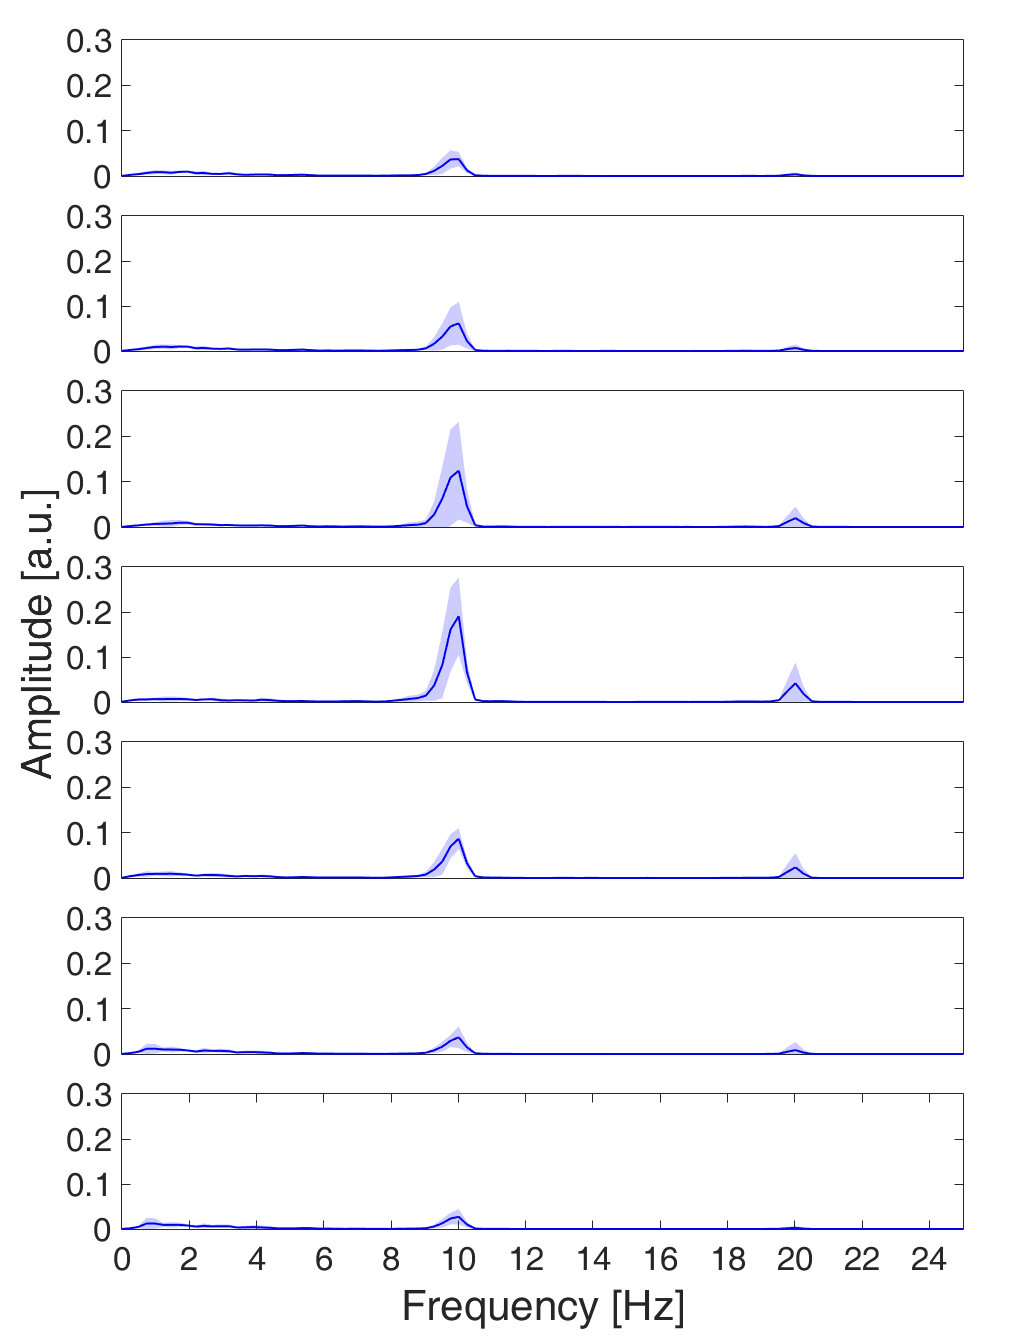
\includegraphics[width=1.\linewidth]{widmo_10Hz.png}
		\caption{Power spectrum for stimulation of 10 Hz.}
		\label{rys:widmo_10Hz}
	\end{subfigure}
	\begin{subfigure}{.5\textwidth}
		\centering
		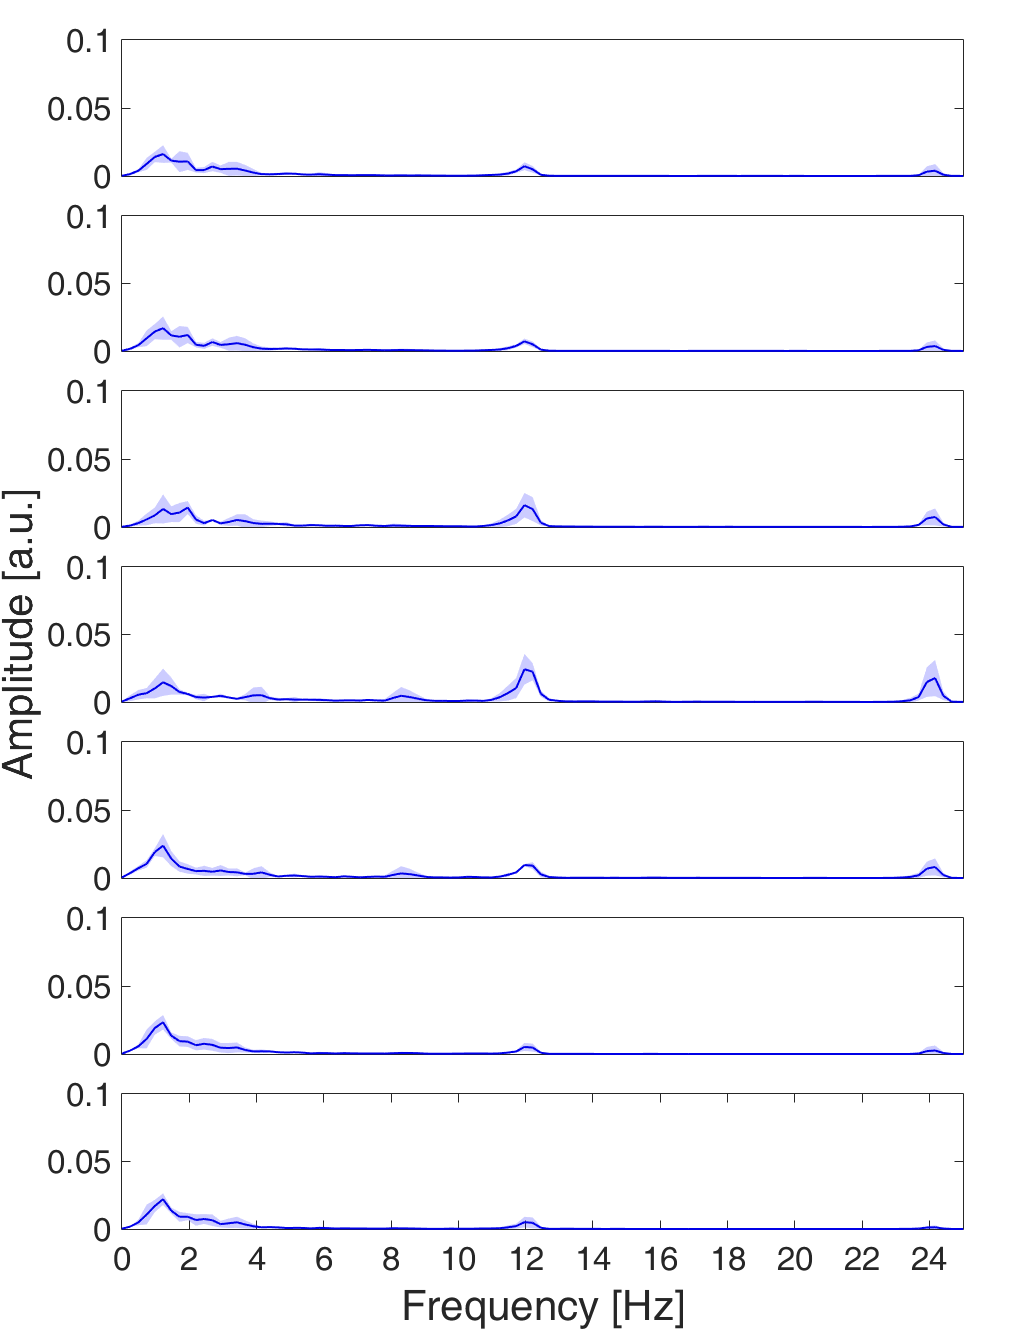
\includegraphics[width=1.\linewidth]{widmo_12Hz.png}
		\caption{Power spectrum for stimulation of 12 Hz.}
		\label{rys:widmo_12Hz}
	\end{subfigure}
	
	\caption{Results in frequency domain for stimulation with high frequencies.}
	\label{rys:srednie_widmo}
	
\end{figure}    
\section{Analysis of current source density}
\label{sec:csd}


Current source density analysis is shown in Figure \ref{rys:csd_1_2} and \ref{rys:csd}. For stimulation of 1 and 2 Hz there is a change in polarization to each repetition of stimulus (Fig.~\ref{rys:csd_1_2}). 

    \begin{figure}[H]
	\begin{subfigure}{.5\textwidth}
		\centering
		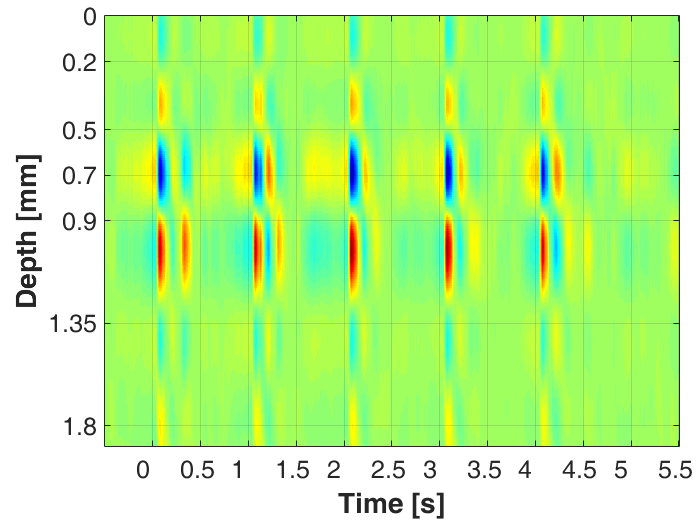
\includegraphics[width=1.\linewidth]{csd_1Hz_5s.png}
		\caption{CSD for stimulation of 1 Hz.}
		\label{rys:csd_1Hz}
	\end{subfigure}
	\begin{subfigure}{.5\textwidth}
		\centering
		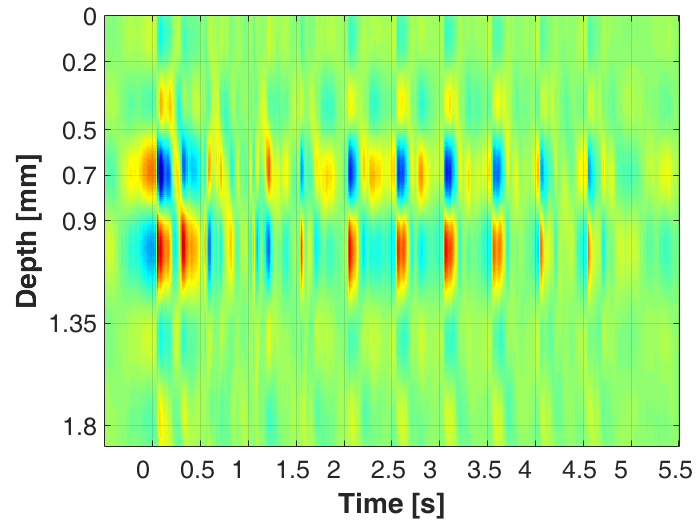
\includegraphics[width=1.\linewidth]{csd_2Hz_5s.png}
		\caption{CSD for stimulation of 2 Hz.}
		\label{rys:csd_2Hz}
	\end{subfigure}
	\begin{subfigure}{\textwidth}
		\centering
		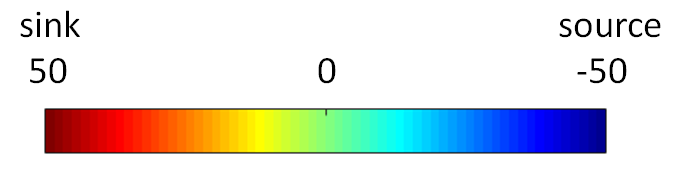
\includegraphics[scale=0.4]{legend2.png}
	\end{subfigure}
	\caption{Results of CSD for stimulation with low frequencies.}
	\label{rys:csd_1_2}
	\end{figure}

For stimulation of frequency higher than 2 Hz there is a change of polarization just after end of stimulation (around 5.2~s; Fig. \ref{rys:csd}). 

	\begin{figure}[H]	
	\begin{subfigure}{.5\textwidth}
		\centering
		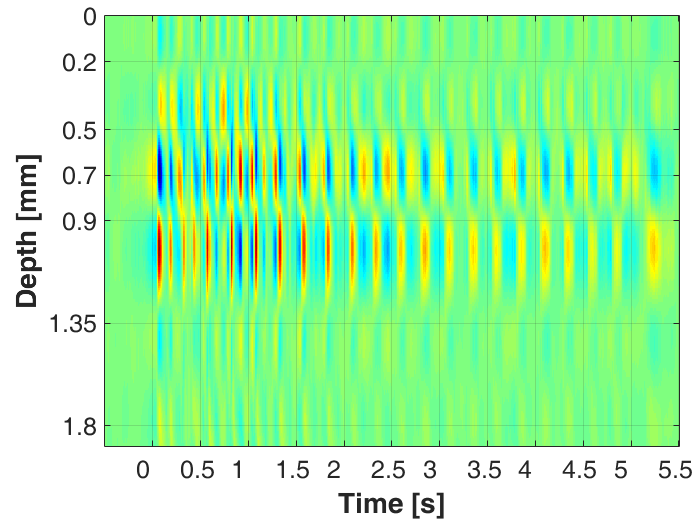
\includegraphics[width=1.\linewidth]{csd_4Hz_5s.png}
		\caption{CSD for stimulation of 4 Hz.}
		\label{rys:csd_4Hz}
	\end{subfigure}
	\begin{subfigure}{.5\textwidth}
		\centering
		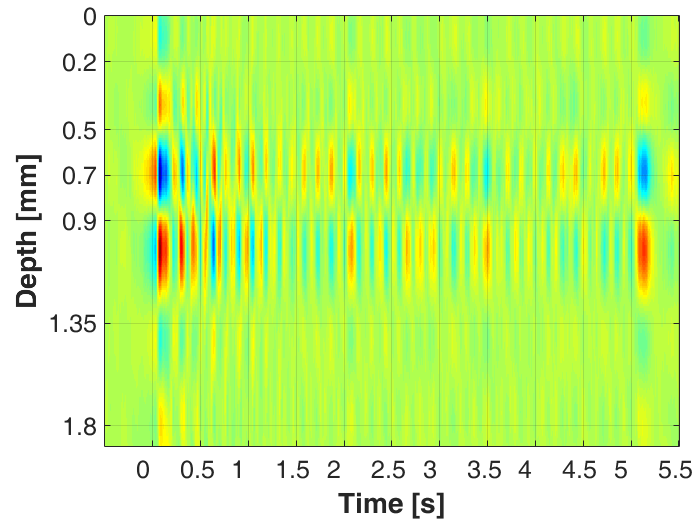
\includegraphics[width=1.\linewidth]{csd_7Hz_5s.png}
		\caption{CSD for stimulation of 7 Hz.}
		\label{rys:csd_7Hz}
	\end{subfigure}
	
	\begin{subfigure}{.5\textwidth}
		\centering
		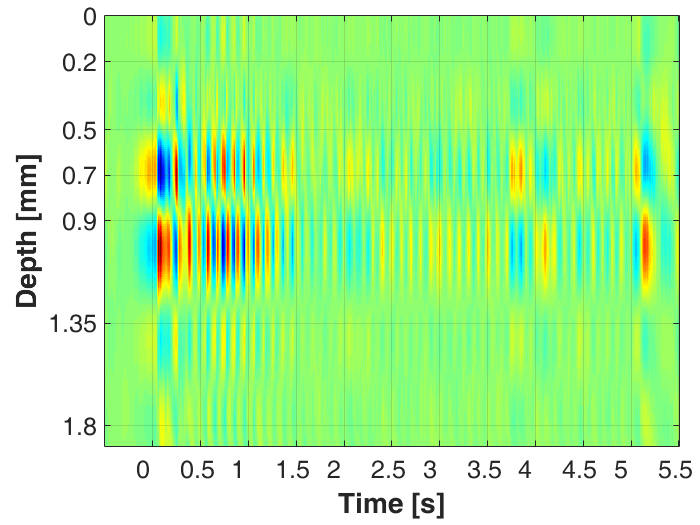
\includegraphics[width=1.\linewidth]{csd_10Hz_5s.png}
		\caption{CSD for stimulation of 10 Hz.}
		\label{rys:csd_10Hz}
	\end{subfigure}
	\begin{subfigure}{.5\textwidth}
		\centering
		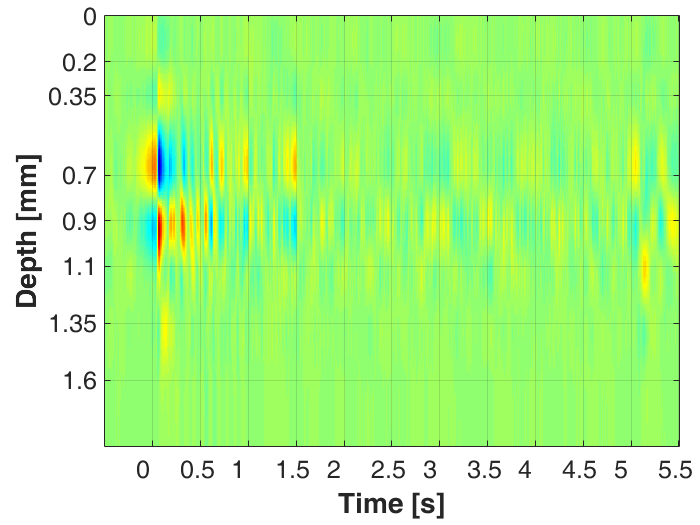
\includegraphics[width=1.\linewidth]{csd_12Hz_5s.png}
		\caption{CSD for stimulation of 12 Hz.}
		\label{rys:csd_12Hz}
	\end{subfigure}
	
	\begin{subfigure}{\textwidth}
	\centering
	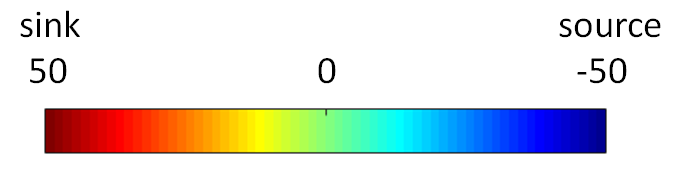
\includegraphics[scale=0.4]{legend2.png}
	\end{subfigure}
	
	\caption{Results of CSD for stimulation with low frequencies.}
	\label{rys:csd}
	
	\end{figure}

    
    \section{Analysis of laminar profile for stimulation with 1 Hz}
        The reverse of potential in layer IV of VCx can be observed (Fig. \ref{rys:srednie_1Hz_1s}). Granular layer (always 4\textsuperscript{th} subfigure) is characterized by the most diverse responses to the stimulation within this group of animals. It can be noticed that first peak of the response is stable whereas second peak is more varied. 
    \begin{figure}[H]
    	\centering
    	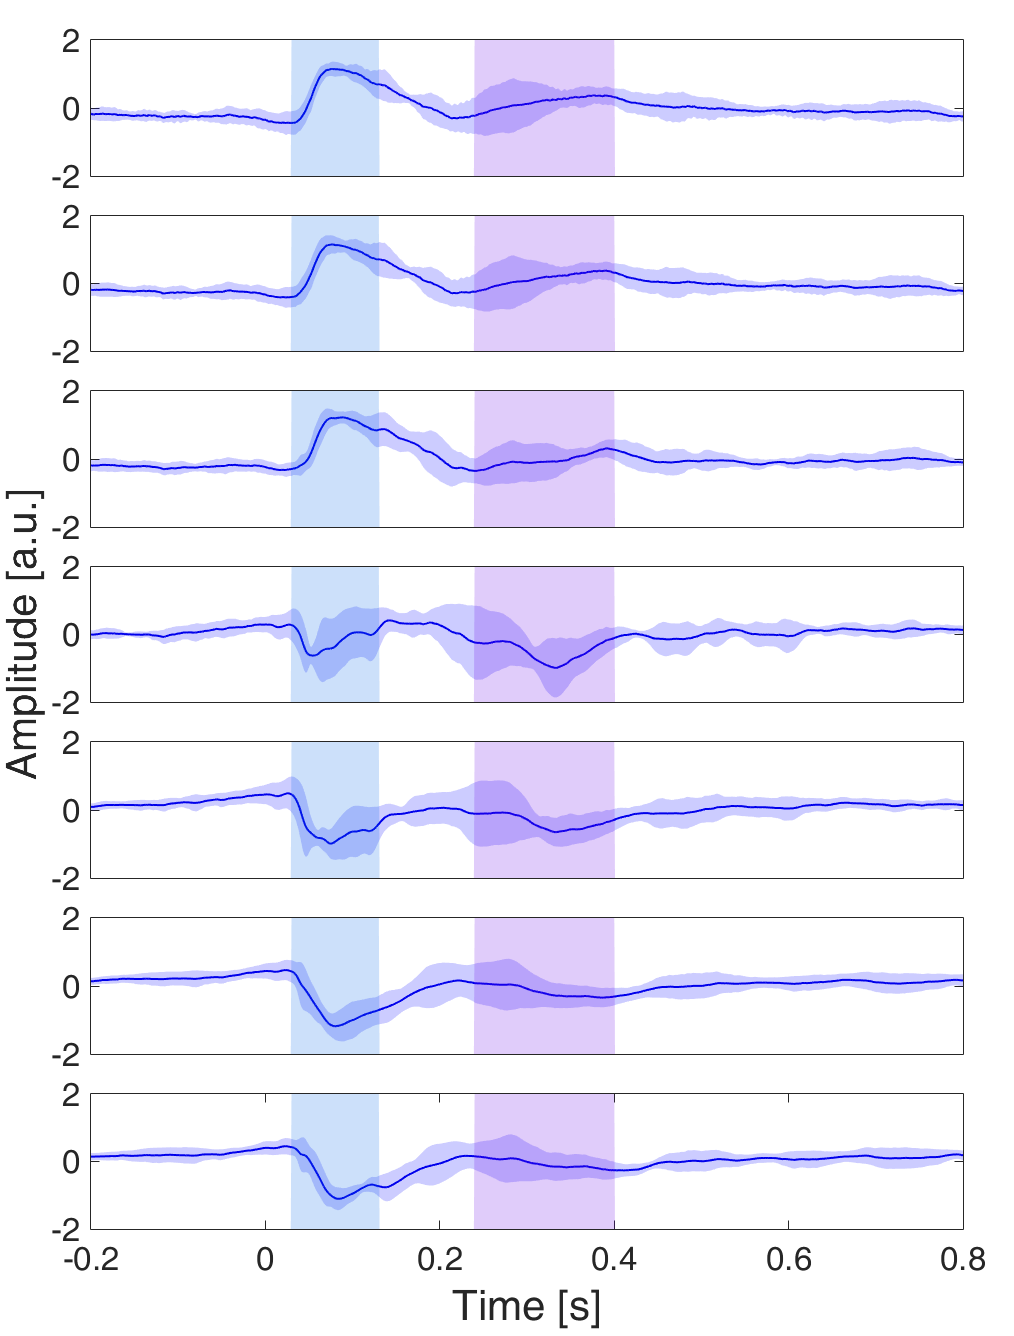
\includegraphics[scale=0.35]{usrednianie_z_tlem.png}
    	\caption{Laminar profile of the response amplitude as a function of depth of the electrode for 1 Hz stimulation. All experiments averaged by 40 trials in time domain---bold line. Differences between animals are by the standard deviation. Time 0 s indicates beginning of 5 s constant stimulation (here only 0.8 s is shown). First and second peak are marked by blue and purple background respectively.}
    	\label{rys:srednie_1Hz_1s}
    \end{figure}
    
     In Figure \ref{rys:profil_1Hz_amp} laminar profile of amplitude of the response in dependence of depth of the electrode is shown. Amplitude of the first peak is very similar among animals and there is a clear change of the sign between the third and the forth channel (Fig. \ref{rys:profil_1Hz_amp1}). Amplitude of the second peak is characterized by a high variance and there is no difference between layers (Fig. \ref{rys:profil_1Hz_amp2}).
     
    \begin{figure}[H]
    	\begin{subfigure}{.5\textwidth}
    		\centering
    		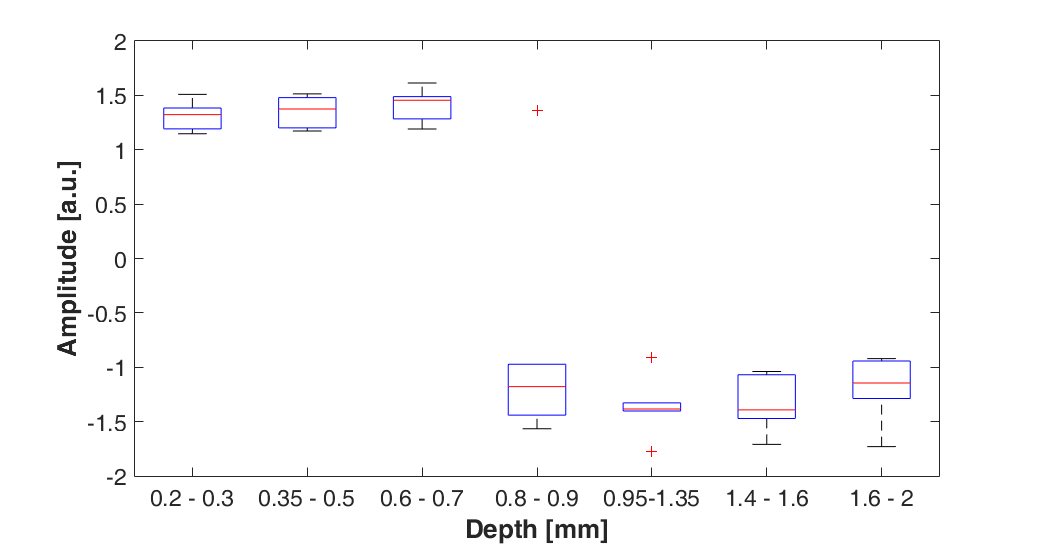
\includegraphics[width=1.\linewidth]{profile_1Hz_amp.png}
    		\caption{Amplitude of the first peak.}
    		\label{rys:profil_1Hz_amp1}
    	\end{subfigure}%
    	\begin{subfigure}{.5\textwidth}
    		\centering
    		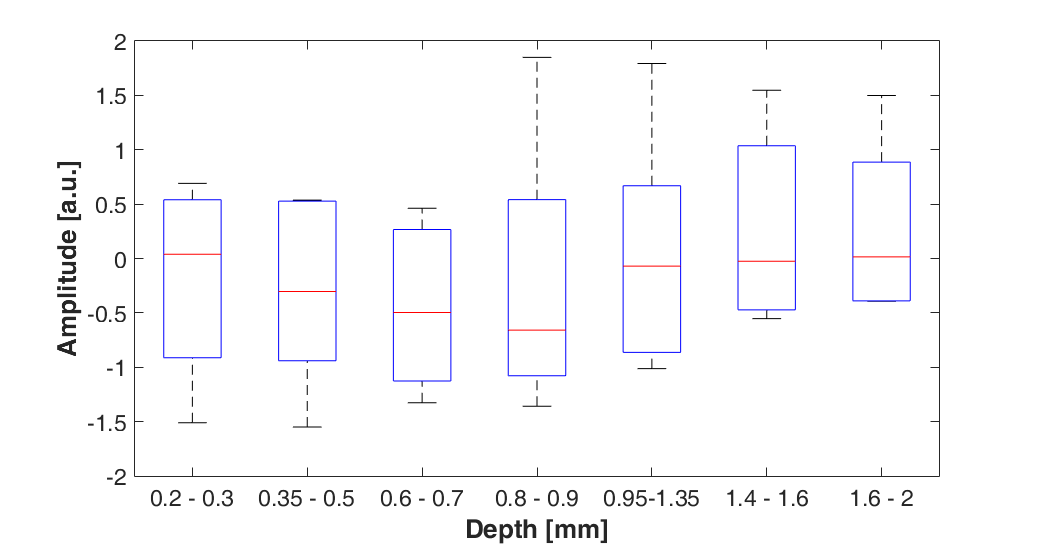
\includegraphics[width=1.\linewidth]{profile_1Hz_amp2.png}
    		\caption{Amplitude of the second peak.}
    		\label{rys:profil_1Hz_amp2}
    	\end{subfigure}
    	
    	\caption{Distribution of amplitudes of the first (a) and the second (b) peak across animals as a function of depth of the electrode for 1~Hz stimulation. On each box, the central mark indicates the median, and the bottom and top edges of the box indicate the 25\textsuperscript{th} and 75\textsuperscript{th} percentiles, respectively. The whiskers extend to the most extreme data points not considering outliers, and the outliers are plotted with red plus.}
    	\label{rys:profil_1Hz_amp}
    \end{figure}


    
    
    In Figure \ref{rys:profil_1Hz_wid} laminar profile of amplitude of the peak fundamental frequency and second harmonic in dependence of depth of the electrode is shown. Amplitude of the first peak is biggest for the fifth channel (Fig. \ref{rys:profil_1Hz_wid1}). Amplitude of the second peak is constant for all channels except for the fourth one. This channel also has the highest variance (Fig.~\ref{rys:profil_1Hz_wid2}).
    
    
    \begin{figure}[H]
    	\begin{subfigure}{.5\textwidth}
    		\centering
    		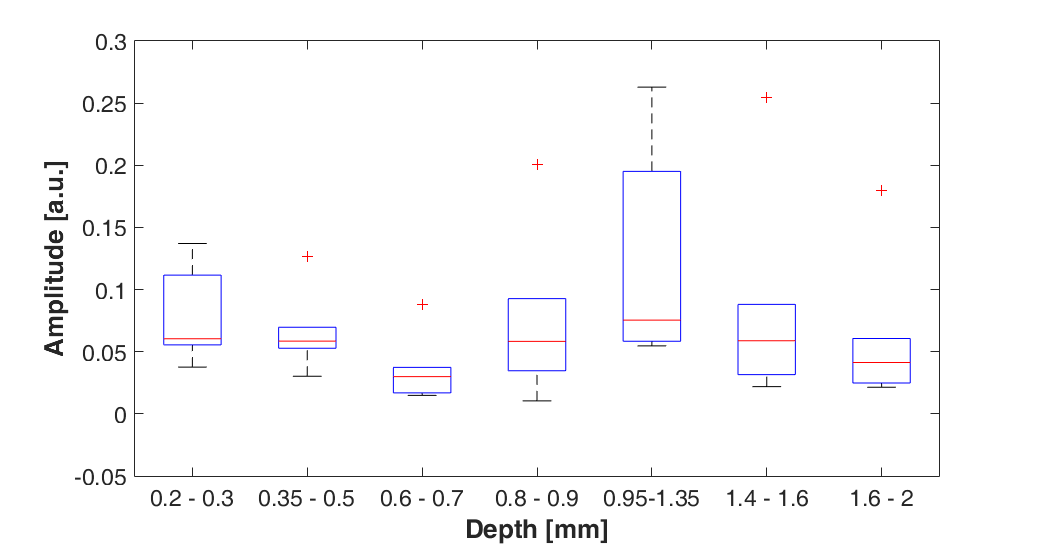
\includegraphics[width=1.\linewidth]{profile_1Hz_wid.png}
    		\caption{Fundamental frequency.}
    		\label{rys:profil_1Hz_wid1}
    	\end{subfigure}%
    	\begin{subfigure}{.5\textwidth}
    		\centering
    		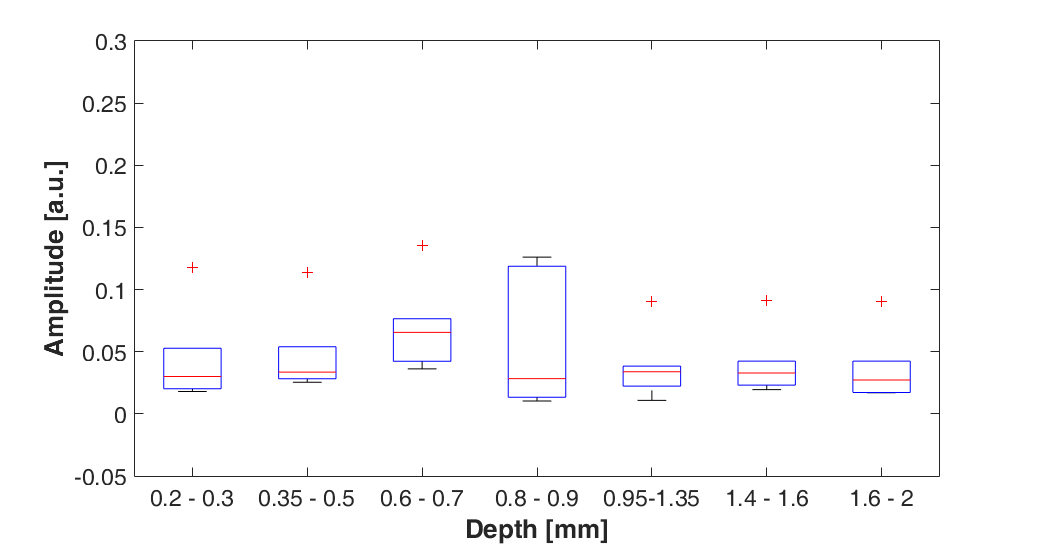
\includegraphics[width=1.\linewidth]{profile_1Hz_wid2.png}
    		\caption{Second harmonic.}
    		\label{rys:profil_1Hz_wid2}
    	\end{subfigure}
    	
    	\caption{Distribution of the amplitude of power spectrum for fundamental frequency (a) and second harmonic (b) as a function of depth of the electrode for 1~Hz stimulation. Meaning of colors and symbols is the same as in Fig.~\ref{rys:profil_1Hz_amp}.}
    	\label{rys:profil_1Hz_wid}
    \end{figure}
    
 
 \section{Analysis of laminar profile for stimulation with 2 Hz}
  
    In the Figure \ref{rys:profil_2Hz_amp} laminar profile of amplitude of response to stimulus in dependence of depth of the electrode for stimulation of 2 Hz is shown. Amplitude of the first peak is very similar among animals except channel 4 where variance is the biggest. (Fig. \ref{rys:profil_2Hz_amp1}). Tendency of amplitude of the second peak is like for 1 Hz: it has a high variance and there is not difference between layers (Fig. \ref{rys:profil_2Hz_amp2}).
  
 	\begin{figure}[H]
 	\begin{subfigure}{.5\textwidth}
 		\centering
 		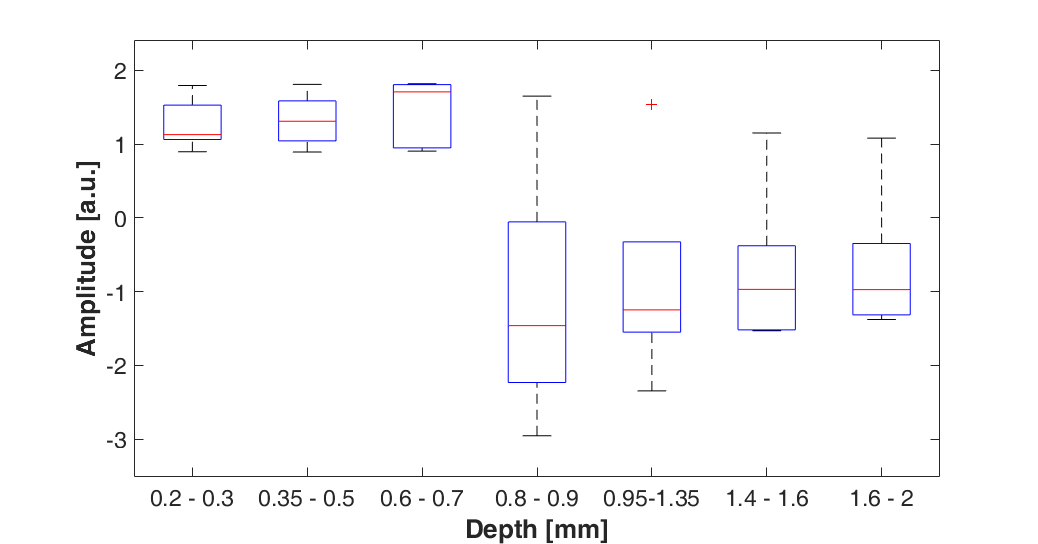
\includegraphics[width=1.\linewidth]{profile_2Hz_amp.png}
 		\caption{Amplitude of the first peak.}
 		\label{rys:profil_2Hz_amp1}
 	\end{subfigure}%
 	\begin{subfigure}{.5\textwidth}
 		\centering
 		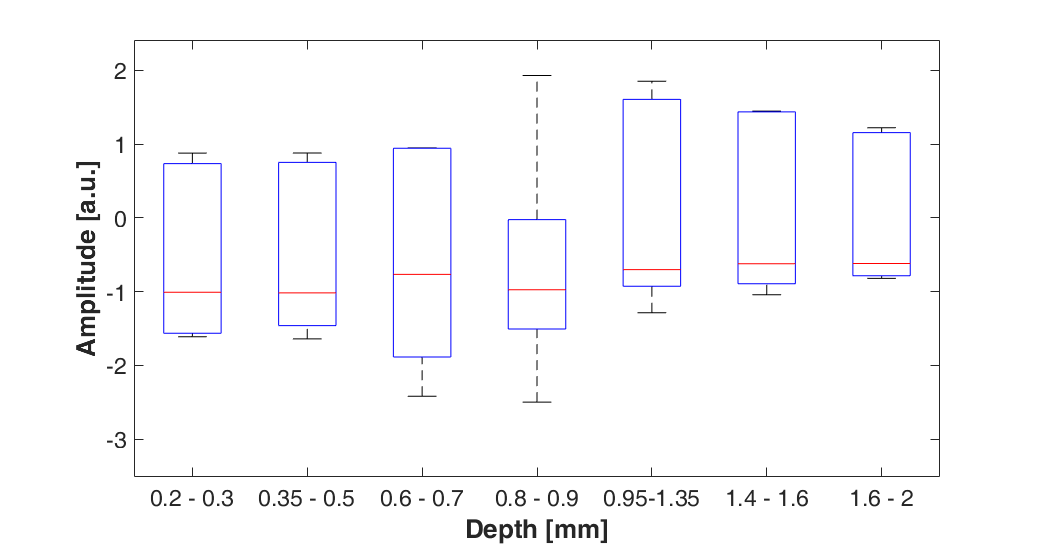
\includegraphics[width=1.\linewidth]{profile_2Hz_amp2.png}
 		\caption{Amplitude of the second peak.}
 		\label{rys:profil_2Hz_amp2}
 	\end{subfigure}
 	
 	\caption{Distribution of amplitudes of the first (a) and the second (b) peak across animals as a function of depth of the electrode for 2~Hz stimulation. Meaning of colors and symbols is the same as in Fig.~\ref{rys:profil_1Hz_amp}.}
 	\label{rys:profil_2Hz_amp}
 \end{figure}

 In the Figure \ref{rys:profil_2Hz_wid} laminar profile of amplitude of peak in 2 and 4 Hz in dependence of depth of the electrode for stimulation of 2 Hz is shown. There is no clear difference for amplitude of the first peak. (Fig. \ref{rys:profil_2Hz_wid1}). Median for second peak is the lowest for forth channel but all channels have the same, high variance (Fig. \ref{rys:profil_2Hz_wid2}).
 
   	\begin{figure}[H]
  	\begin{subfigure}{.5\textwidth}
  		\centering
  		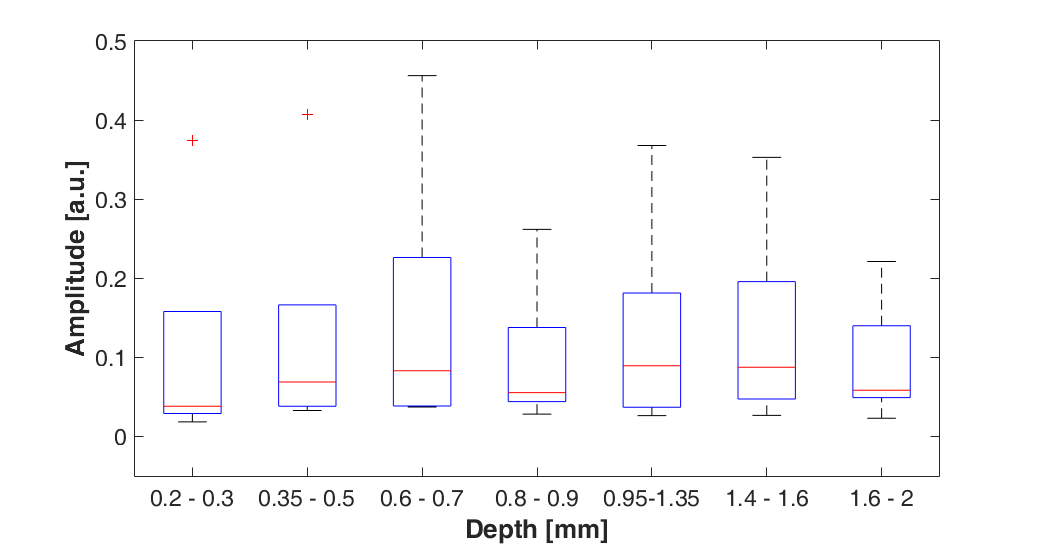
\includegraphics[width=1.\linewidth]{profile_2Hz_wid.png}
  		\caption{Fundamental frequency.}
  		\label{rys:profil_2Hz_wid1}
  	\end{subfigure}%
  	\begin{subfigure}{.5\textwidth}
  		\centering
  		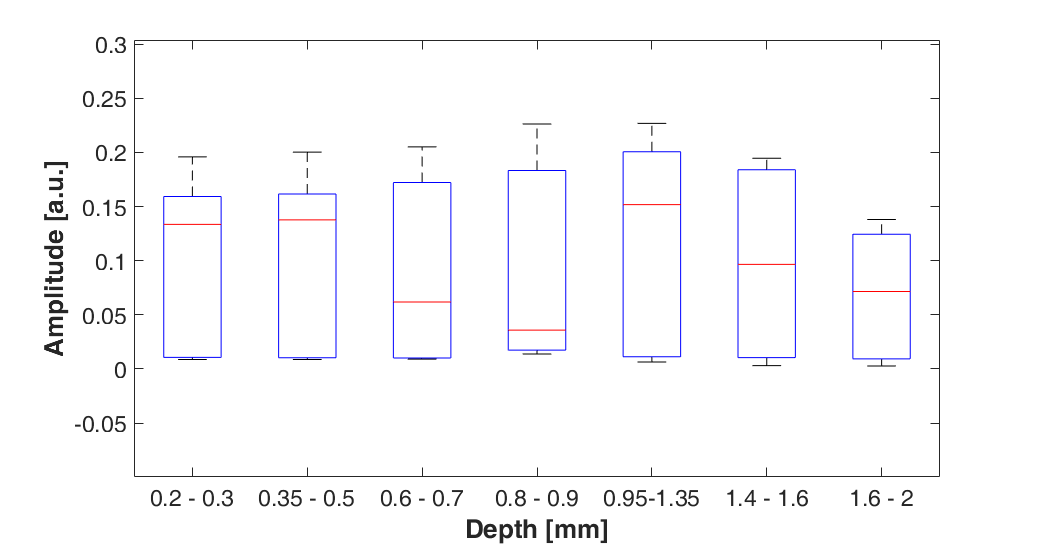
\includegraphics[width=1.\linewidth]{profile_2Hz_wid2.png}
  		\caption{Second harmonic.}
  		\label{rys:profil_2Hz_wid2}
  	\end{subfigure}
  	
  	\caption{Distribution of the amplitude of power spectrum for fundamental frequency (a) and second harmonic (b) as a function of depth of the electrode for 2~Hz stimulation. Meaning of colors and symbols is the same as in Fig.~\ref{rys:profil_1Hz_amp}.}
  	\label{rys:profil_2Hz_wid}
  \end{figure}

  
\section{Analysis of laminar profile for stimulation with 4 Hz} 

 In the Figure \ref{rys:profil_4Hz_wid} laminar profile of amplitude of peak in 4 and 8 Hz in dependence of depth of the electrode for stimulation of 4 Hz is shown. For both frequencies median has the biggest value for forth channel. The following tendency could be observed: upper- and lowermost channels exhibit low amplitudes, while highest amplitudes are reached in the middle channels. 

   	\begin{figure}[H]
	\begin{subfigure}{.5\textwidth}
		\centering
		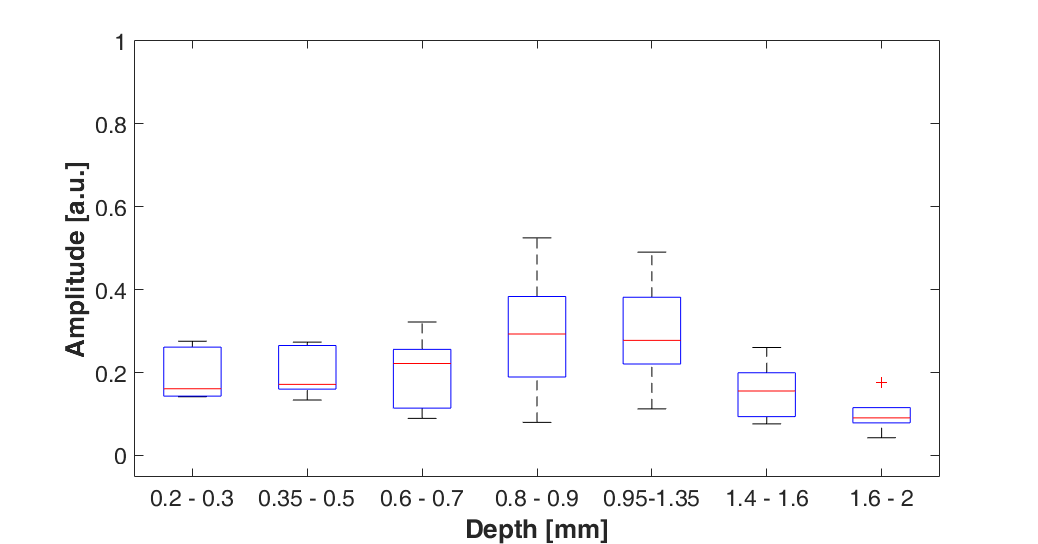
\includegraphics[width=1.\linewidth]{profile_4Hz_wid.png}
		\caption{}
		\label{rys:profil_4Hz_wid1}
	\end{subfigure}%
	\begin{subfigure}{.5\textwidth}
		\centering
		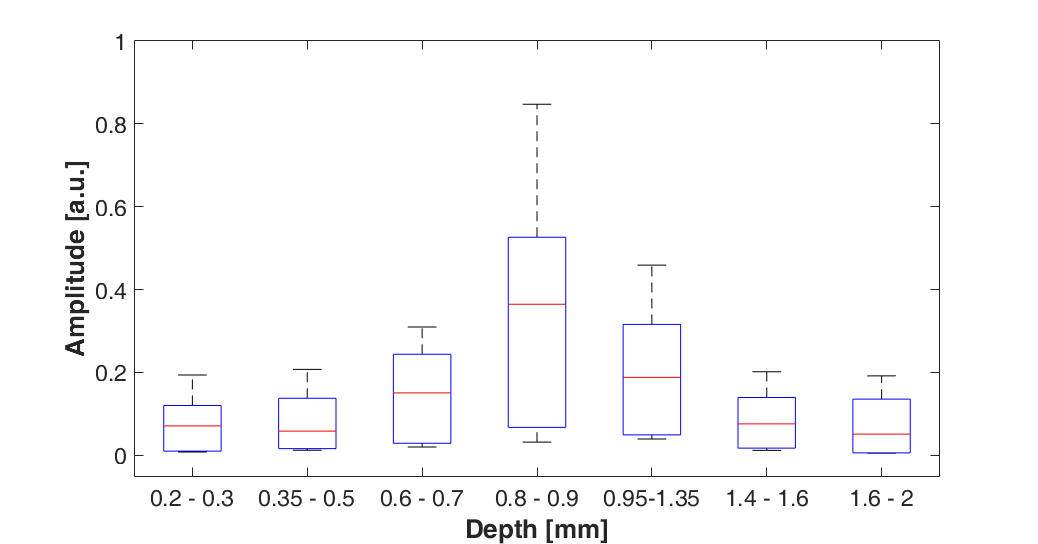
\includegraphics[width=1.\linewidth]{profile_4Hz_wid2.png}
		\caption{}
		\label{rys:profil_4Hz_wid2}
	\end{subfigure}
	\caption{Distribution of the amplitude of power spectrum for fundamental frequency (a) and second harmonic (b) as a function of depth of the electrode for 4~Hz stimulation. Meaning of colors and symbols is the same as in Fig.~\ref{rys:profil_1Hz_amp}.}
	\label{rys:profil_4Hz_wid}
\end{figure}

\section{Analysis of laminar profile for stimulation with 7 Hz}  

In the Figure \ref{rys:profil_7Hz_wid} laminar profile of amplitude of peak in 7 and 14 Hz in dependence of depth of the electrode for stimulation of 7 Hz is shown. As well as for 4 Hz, in the stimulation with 7 Hz the biggest median is for forth channel. But due to high variance for distribution of the amplitude of fundamental frequency only for second harmonic there is the same tendency  as observed for 4 Hz.


   	\begin{figure}[H]
	\begin{subfigure}{.5\textwidth}
		\centering
		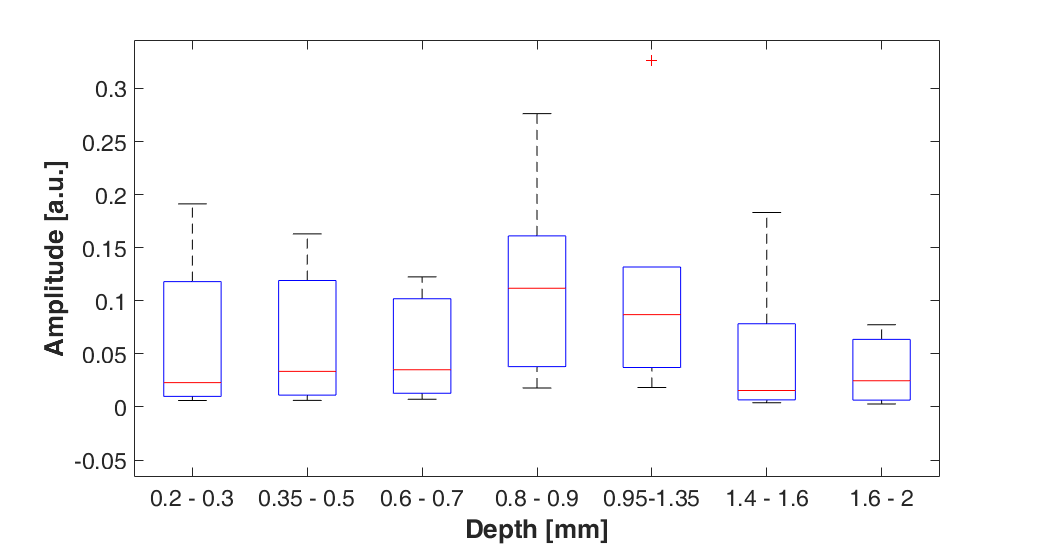
\includegraphics[width=1.\linewidth]{profile_7Hz_wid.png}
		\caption{}
		\label{rys:profil_7Hz_wid1}
	\end{subfigure}%
	\begin{subfigure}{.5\textwidth}
		\centering
		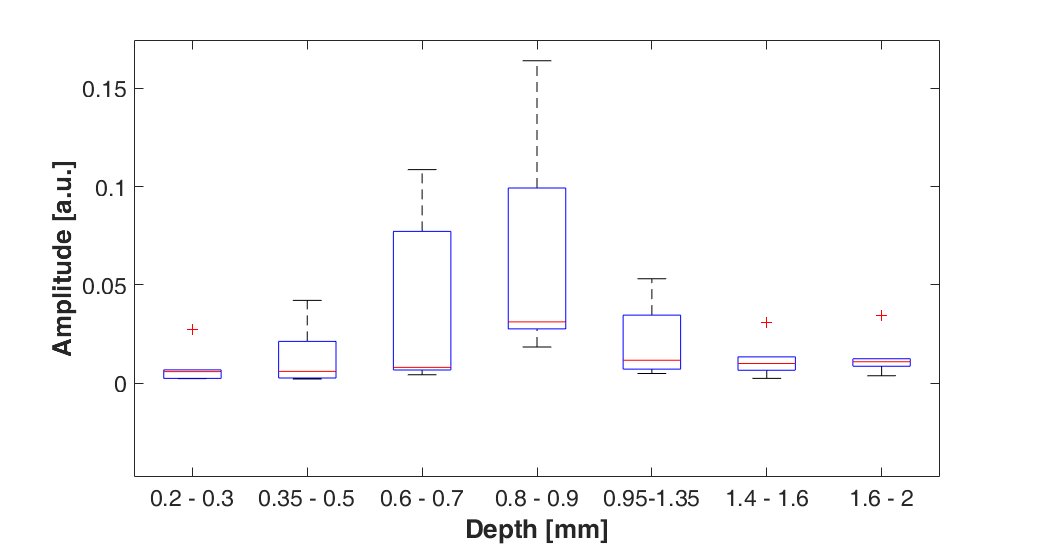
\includegraphics[width=1.\linewidth]{profile_7Hz_wid2.png}
		\caption{}
		\label{rys:profil_7Hz_wid2}
	\end{subfigure}
	\caption{Distribution of the amplitude of power spectrum for fundamental frequency (a) and second harmonic (b) as a function of depth of the electrode for 7~Hz stimulation. Meaning of colors and symbols is the same as in Fig.~\ref{rys:profil_1Hz_amp}.}
	\label{rys:profil_7Hz_wid}
\end{figure}
\section{Analysis of laminar profile for stimulation with 10 Hz}  

In the Figure \ref{rys:profil_10Hz_wid} laminar profile of amplitude of peak in 10 and 20 Hz in dependence of depth of the electrode for stimulation of 10 Hz is shown. For both fundamental frequency and second harmonic there is clear tendency as for 4 Hz--- the highest amplitude is for forth channel and the farther channel is from the middle has the lower amplitude.

   	\begin{figure}[H]
	\begin{subfigure}{.5\textwidth}
		\centering
		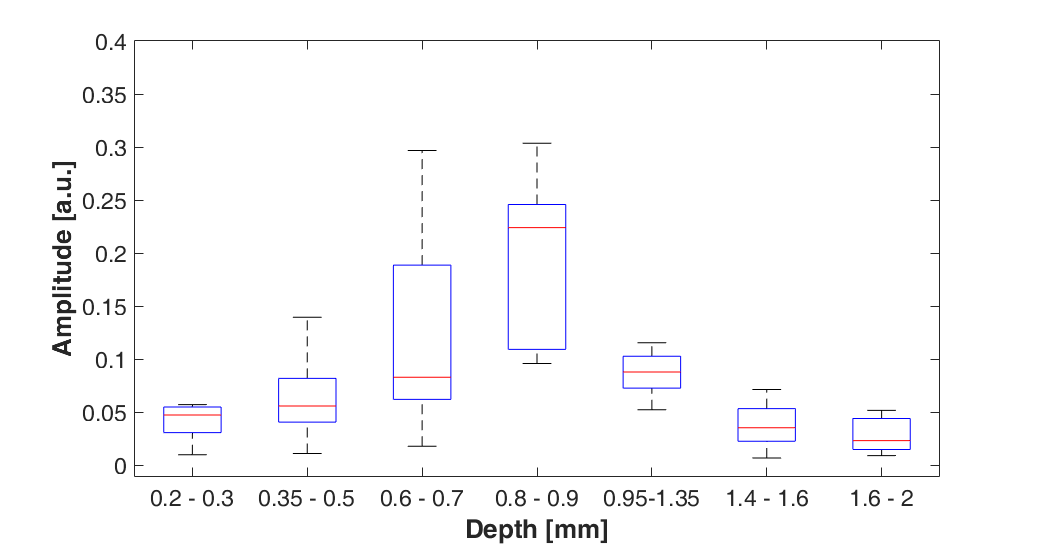
\includegraphics[width=1.\linewidth]{profile_10Hz_wid.png}
		\caption{}
		\label{rys:profil_10Hz_wid1}
	\end{subfigure}%
	\begin{subfigure}{.5\textwidth}
		\centering
		\includegraphics[width=1.\linewidth]{profile_10Hz_wid2.png}
		\caption{}
		\label{rys:profil_10Hz_wid2}
	\end{subfigure}
	\caption{Distribution of the amplitude of power spectrum for fundamental frequency (a) and second harmonic (b) as a function of depth of the electrode for 10~Hz stimulation. Meaning of colors and symbols is the same as in Fig.~\ref{rys:profil_1Hz_amp}.}
	\label{rys:profil_10Hz_wid}
\end{figure}
\section{Analysis of laminar profile for stimulation with 12 Hz}  
In the Figure \ref{rys:profil_12Hz_wid} laminar profile of amplitude of peak in 12 and 24 Hz in dependence of depth of the electrode for stimulation of 12 Hz is shown. For both frequencies tendency is the same as for the other stimulations with high frequencies.

   	\begin{figure}[H]
	\begin{subfigure}{.5\textwidth}
		\centering
		\includegraphics[width=1.\linewidth]{profile_12Hz_wid.png}
		\caption{}
		\label{rys:profil_12Hz_wid1}
	\end{subfigure}%
	\begin{subfigure}{.5\textwidth}
		\centering
		\includegraphics[width=1.\linewidth]{profile_12Hz_wid2.png}
		\caption{}
		\label{rys:profil_12Hz_wid2}
	\end{subfigure}
	\caption{Distribution of the amplitude of power spectrum for fundamental frequency (a) and second harmonic (b) as a function of depth of the electrode for 12~Hz stimulation. Meaning of colors and symbols is the same as in Fig.~\ref{rys:profil_1Hz_amp}.}
	\label{rys:profil_12Hz_wid}
\end{figure}
    \chapter{Discussion}
    In this work responses to visual stimulation with 6 different temporal frequencies from range 1--12 Hz on 6 Wistar rats were studied. Results were presented as averaged potentials, power spectra and current source density, which allowed to find differences in laminar profile.
    
    It is worth mentioning that even though all recordings were performed on the same structure, using the same electrode, brain anatomy differs between subjects. Individual channels were chosen for analysis based on the pattern of visual potential so there is no guarantee that one channel represents exactly the same location for every animal. The same concerns the method of recording signal---local field potential is a spatially inaccurate method because it gathers signal from quite a big area of the brain. On the other hand, this experiment was performed on a group of six animals and the obtained results are coherent and repeatable. Especially the latter confirms that the conclusions are correct. 
    
    Analysis in time domain for low frequencies seems to be adequate, as it was observed that only for stimulus with intervals longer than 400 ms the response to second repetition of stimulus is as strong as to the first one (\cite{retino}).
    
    Analysis of averaged signal for 1 Hz and 2 Hz indicates that there is a clear difference in amplitude of the first peak between supra- and infragranular layers. Supragranular layers are characterized by positive amplitude, while infragranular by negative. It can be a result of the fact that magnocellular channel enters from LGN mainly to layer IV of VCx. For both 1 Hz and 2 Hz stimulations there was a high variance of the amplitude of the second peak between animals. Although the results of averaged potentials are similar for both low-frequency stimulations, there are substantial differences in the peaks for fundamental frequency and second harmonic. For 1 Hz stimulation channel 5 exhibited the highest amplitude and variance of fundamental frequency, while for 2 Hz stimulation channel 4 had the lowest value and variance. The same concerns the second harmonic: for 1 Hz stimulation all channels had similar values except channel 4 which stood out having the highest variance. For 2 Hz stimulation the situation was quite opposite---channel 4 exhibited the lowest variance. Those contradictory effects may be a result of improper method of analysis. On the other hand, they could be due to high amplitude of low frequencies which are present in a sleeping animal so that low frequency of stimulation may be not enough to stand out (\cite{sellers, ja}).
    
    For stimulation with frequency higher than 2 Hz the signal forms a continuous oscillation. The amplitude of these oscillations during the first 1.5 s is higher than for the rest of the stimulation. Due to lack of clear peaks after stimuli analysis of evoked potentials could not be performed. The analysis in the frequency domain the same tendency for all frequencies was observed: channel 4 is characterized by the highest amplitude and has lower variance than other channels; upper- and lowermost channels exhibit the lowest amplitudes. This tendency is noticeable for fundamental frequency, but for second harmonic it is much more apparent. It may be a result of magnocellular entrance in layer IV in VCx.
    
    Results obtained for CSD are consistent with study on macaque VCx (\cite{maier2011}). Although the authors used a longer flash (100-ms-long flashing screen) they also observed the initial current sink in response to the stimulus in layer IV. Unfortunately that study analyzed only on first 0.2~s after stimulus so the rest of the data could not be compared with our results. 
    
    CSD analysis of low frequency stimulation revealed a clear sink and source after every stimulus and the observed response is consistent with other results (\cite{kozai, maier2010}). In case of high frequencies current flows could be observed only during the first 1.5 s of the stimulation, after which a silencing occurs. Just after the stimulation a big difference in polarization was noticed, which could be due to a suppression resulting from a very strong stimulus.
    

\printbibliography[heading=bibintoc]

\end{document}
